% Options for packages loaded elsewhere
\PassOptionsToPackage{unicode}{hyperref}
\PassOptionsToPackage{hyphens}{url}
%
\documentclass[
]{article}
\usepackage{lmodern}
\usepackage{amssymb,amsmath}
\usepackage{ifxetex,ifluatex}
\ifnum 0\ifxetex 1\fi\ifluatex 1\fi=0 % if pdftex
  \usepackage[T1]{fontenc}
  \usepackage[utf8]{inputenc}
  \usepackage{textcomp} % provide euro and other symbols
\else % if luatex or xetex
  \usepackage{unicode-math}
  \defaultfontfeatures{Scale=MatchLowercase}
  \defaultfontfeatures[\rmfamily]{Ligatures=TeX,Scale=1}
\fi
% Use upquote if available, for straight quotes in verbatim environments
\IfFileExists{upquote.sty}{\usepackage{upquote}}{}
\IfFileExists{microtype.sty}{% use microtype if available
  \usepackage[]{microtype}
  \UseMicrotypeSet[protrusion]{basicmath} % disable protrusion for tt fonts
}{}
\makeatletter
\@ifundefined{KOMAClassName}{% if non-KOMA class
  \IfFileExists{parskip.sty}{%
    \usepackage{parskip}
  }{% else
    \setlength{\parindent}{0pt}
    \setlength{\parskip}{6pt plus 2pt minus 1pt}}
}{% if KOMA class
  \KOMAoptions{parskip=half}}
\makeatother
\usepackage{xcolor}
\IfFileExists{xurl.sty}{\usepackage{xurl}}{} % add URL line breaks if available
\IfFileExists{bookmark.sty}{\usepackage{bookmark}}{\usepackage{hyperref}}
\hypersetup{
  pdftitle={Tipología y Ciclo de Vida de Datos - Práctica 2},
  pdfauthor={aruizplaza \& rcotillas},
  hidelinks,
  pdfcreator={LaTeX via pandoc}}
\urlstyle{same} % disable monospaced font for URLs
\usepackage[margin=1in]{geometry}
\usepackage{color}
\usepackage{fancyvrb}
\newcommand{\VerbBar}{|}
\newcommand{\VERB}{\Verb[commandchars=\\\{\}]}
\DefineVerbatimEnvironment{Highlighting}{Verbatim}{commandchars=\\\{\}}
% Add ',fontsize=\small' for more characters per line
\usepackage{framed}
\definecolor{shadecolor}{RGB}{48,48,48}
\newenvironment{Shaded}{\begin{snugshade}}{\end{snugshade}}
\newcommand{\AlertTok}[1]{\textcolor[rgb]{1.00,0.81,0.69}{#1}}
\newcommand{\AnnotationTok}[1]{\textcolor[rgb]{0.50,0.62,0.50}{\textbf{#1}}}
\newcommand{\AttributeTok}[1]{\textcolor[rgb]{0.80,0.80,0.80}{#1}}
\newcommand{\BaseNTok}[1]{\textcolor[rgb]{0.86,0.64,0.64}{#1}}
\newcommand{\BuiltInTok}[1]{\textcolor[rgb]{0.80,0.80,0.80}{#1}}
\newcommand{\CharTok}[1]{\textcolor[rgb]{0.86,0.64,0.64}{#1}}
\newcommand{\CommentTok}[1]{\textcolor[rgb]{0.50,0.62,0.50}{#1}}
\newcommand{\CommentVarTok}[1]{\textcolor[rgb]{0.50,0.62,0.50}{\textbf{#1}}}
\newcommand{\ConstantTok}[1]{\textcolor[rgb]{0.86,0.64,0.64}{\textbf{#1}}}
\newcommand{\ControlFlowTok}[1]{\textcolor[rgb]{0.94,0.87,0.69}{#1}}
\newcommand{\DataTypeTok}[1]{\textcolor[rgb]{0.87,0.87,0.75}{#1}}
\newcommand{\DecValTok}[1]{\textcolor[rgb]{0.86,0.86,0.80}{#1}}
\newcommand{\DocumentationTok}[1]{\textcolor[rgb]{0.50,0.62,0.50}{#1}}
\newcommand{\ErrorTok}[1]{\textcolor[rgb]{0.76,0.75,0.62}{#1}}
\newcommand{\ExtensionTok}[1]{\textcolor[rgb]{0.80,0.80,0.80}{#1}}
\newcommand{\FloatTok}[1]{\textcolor[rgb]{0.75,0.75,0.82}{#1}}
\newcommand{\FunctionTok}[1]{\textcolor[rgb]{0.94,0.94,0.56}{#1}}
\newcommand{\ImportTok}[1]{\textcolor[rgb]{0.80,0.80,0.80}{#1}}
\newcommand{\InformationTok}[1]{\textcolor[rgb]{0.50,0.62,0.50}{\textbf{#1}}}
\newcommand{\KeywordTok}[1]{\textcolor[rgb]{0.94,0.87,0.69}{#1}}
\newcommand{\NormalTok}[1]{\textcolor[rgb]{0.80,0.80,0.80}{#1}}
\newcommand{\OperatorTok}[1]{\textcolor[rgb]{0.94,0.94,0.82}{#1}}
\newcommand{\OtherTok}[1]{\textcolor[rgb]{0.94,0.94,0.56}{#1}}
\newcommand{\PreprocessorTok}[1]{\textcolor[rgb]{1.00,0.81,0.69}{\textbf{#1}}}
\newcommand{\RegionMarkerTok}[1]{\textcolor[rgb]{0.80,0.80,0.80}{#1}}
\newcommand{\SpecialCharTok}[1]{\textcolor[rgb]{0.86,0.64,0.64}{#1}}
\newcommand{\SpecialStringTok}[1]{\textcolor[rgb]{0.80,0.58,0.58}{#1}}
\newcommand{\StringTok}[1]{\textcolor[rgb]{0.80,0.58,0.58}{#1}}
\newcommand{\VariableTok}[1]{\textcolor[rgb]{0.80,0.80,0.80}{#1}}
\newcommand{\VerbatimStringTok}[1]{\textcolor[rgb]{0.80,0.58,0.58}{#1}}
\newcommand{\WarningTok}[1]{\textcolor[rgb]{0.50,0.62,0.50}{\textbf{#1}}}
\usepackage{longtable,booktabs}
% Correct order of tables after \paragraph or \subparagraph
\usepackage{etoolbox}
\makeatletter
\patchcmd\longtable{\par}{\if@noskipsec\mbox{}\fi\par}{}{}
\makeatother
% Allow footnotes in longtable head/foot
\IfFileExists{footnotehyper.sty}{\usepackage{footnotehyper}}{\usepackage{footnote}}
\makesavenoteenv{longtable}
\usepackage{graphicx,grffile}
\makeatletter
\def\maxwidth{\ifdim\Gin@nat@width>\linewidth\linewidth\else\Gin@nat@width\fi}
\def\maxheight{\ifdim\Gin@nat@height>\textheight\textheight\else\Gin@nat@height\fi}
\makeatother
% Scale images if necessary, so that they will not overflow the page
% margins by default, and it is still possible to overwrite the defaults
% using explicit options in \includegraphics[width, height, ...]{}
\setkeys{Gin}{width=\maxwidth,height=\maxheight,keepaspectratio}
% Set default figure placement to htbp
\makeatletter
\def\fps@figure{htbp}
\makeatother
\setlength{\emergencystretch}{3em} % prevent overfull lines
\providecommand{\tightlist}{%
  \setlength{\itemsep}{0pt}\setlength{\parskip}{0pt}}
\setcounter{secnumdepth}{-\maxdimen} % remove section numbering

\title{Tipología y Ciclo de Vida de Datos - Práctica 2}
\author{aruizplaza \& rcotillas}
\date{10/12/2020}

\begin{document}
\maketitle

{
\setcounter{tocdepth}{2}
\tableofcontents
}
\hypertarget{descripciuxf3n-del-dataset.-por-quuxe9-es-importante-y-quuxe9-preguntaproblema-pretende-responder}{%
\section{.- Descripción del dataset. ¿Por qué es importante y qué
pregunta/problema pretende
responder?}\label{descripciuxf3n-del-dataset.-por-quuxe9-es-importante-y-quuxe9-preguntaproblema-pretende-responder}}

La importancia de este dataset se puede explicar desde un punto de vista
histórico (periodístico, documental, etc.), así como desde un punto de
vista socioeconómico. En cuanto al primero, el suceso al que está
vinculado este conjunto de datos, fue uno de los accidentes más
impactantes del siglo pasado y el estudio de los datos puede ayudar a
entender un poco mejor que ocurrió, al menos en lo referente a lo que la
supervivencia se refiere. En cuanto al segundo, el estudio de este
dataset nos puede ayudar a encontrar patrones que pueden repetirse en
situaciones similares, así como estudiar si la pertencencia a cierta
clase o género otorga o no ventajas ante este tipo de situaciones.

En esta práctica trataremos de responder a las siguientes preguntas:

\begin{enumerate}
\def\labelenumi{(\arabic{enumi})}
\item
  ¿Se puede predecir la supervivencia?
\item
  ¿Que tratamiento de nulos en la variable edad se comporta mejor en la
  prediccion de la supervivencia?
\item
  ¿Que variables influyen mas en la supervivencia?
\item
  ¿la supervivencia es mayor en caso de ser niño o mujer?
\end{enumerate}

\hypertarget{integraciuxf3n-y-selecciuxf3n-de-los-datos-de-interuxe9s-a-analizar.}{%
\section{.- Integración y selección de los datos de interés a
analizar.}\label{integraciuxf3n-y-selecciuxf3n-de-los-datos-de-interuxe9s-a-analizar.}}

\begin{quote}
Instalación y Llamada de los paquetes a utilizar durante la práctica
\end{quote}

\begin{Shaded}
\begin{Highlighting}[]
\CommentTok{# Cargamos paquete TIDYVERSE que engloba a otros paquetes que nos permiten llevar a cabo la importación, transformación, visualización, modelado y comunicación de datos/información}
\ControlFlowTok{if}\NormalTok{(}\OperatorTok{!}\KeywordTok{require}\NormalTok{(tidyverse))\{}
    \KeywordTok{install.packages}\NormalTok{(}\StringTok{'tidyverse'}\NormalTok{, }\DataTypeTok{repos=}\StringTok{'http://cran.us.r-project.org'}\NormalTok{)}
\NormalTok{\}}
\KeywordTok{library}\NormalTok{(tidyverse)}

\CommentTok{# Cargamos paquete PSYCH que agrupa funciones  utilizadas en psicología.}
\ControlFlowTok{if}\NormalTok{(}\OperatorTok{!}\KeywordTok{require}\NormalTok{(psych))\{}
    \KeywordTok{install.packages}\NormalTok{(}\StringTok{'psych'}\NormalTok{, }\DataTypeTok{repos=}\StringTok{'http://cran.us.r-project.org'}\NormalTok{)}
\NormalTok{\}}
\KeywordTok{library}\NormalTok{(psych)}

\CommentTok{# Cargamos paquete reticulate proporciona un conjunto de  herramientas para integrar código Python y R.}
\ControlFlowTok{if}\NormalTok{(}\OperatorTok{!}\KeywordTok{require}\NormalTok{(reticulate))\{}
    \KeywordTok{install.packages}\NormalTok{(}\StringTok{'reticulate'}\NormalTok{, }\DataTypeTok{repos=}\StringTok{'http://cran.us.r-project.org'}\NormalTok{)}
\NormalTok{\}}
\KeywordTok{library}\NormalTok{(reticulate)}

\CommentTok{# Cargamos paquete CORRPLOT nos permite la representación gráfica de una matriz de correlación, así como nos proporciona algunos algoritmos para hacer reordenamiento de la matriz}
\ControlFlowTok{if}\NormalTok{(}\OperatorTok{!}\KeywordTok{require}\NormalTok{(corrplot))\{}
    \KeywordTok{install.packages}\NormalTok{(}\StringTok{'corrplot'}\NormalTok{, }\DataTypeTok{repos=}\StringTok{'http://cran.us.r-project.org'}\NormalTok{)}
\NormalTok{\}}
\KeywordTok{library}\NormalTok{(corrplot)}

\CommentTok{# Cargamos paquete DESCTOOLS que proporciona una colección de funciones estadísticas básicas para la descripción de datos}
\ControlFlowTok{if}\NormalTok{(}\OperatorTok{!}\KeywordTok{require}\NormalTok{(DescTools))\{}
    \KeywordTok{install.packages}\NormalTok{(}\StringTok{'DescTools'}\NormalTok{, }\DataTypeTok{repos=}\StringTok{'http://cran.us.r-project.org'}\NormalTok{)}
\NormalTok{\}}
\KeywordTok{library}\NormalTok{(DescTools)}

\CommentTok{# Cargamos paquete ARULES que proporciona la infraestructura para representar, manipular y analizar los datos y patrones de las transacciones (conjuntos de elementos frecuentes y reglas de asociación)}
\ControlFlowTok{if}\NormalTok{(}\OperatorTok{!}\KeywordTok{require}\NormalTok{(arules))\{}
    \KeywordTok{install.packages}\NormalTok{(}\StringTok{'arules'}\NormalTok{, }\DataTypeTok{repos=}\StringTok{'http://cran.us.r-project.org'}\NormalTok{)}
\NormalTok{\}}
\KeywordTok{library}\NormalTok{(arules)}

\CommentTok{# Cargamos paquete CLUSTER que nos proporciona métodos de análisis de clusters (Agrupaciones)}
\ControlFlowTok{if}\NormalTok{(}\OperatorTok{!}\KeywordTok{require}\NormalTok{(cluster))\{}
    \KeywordTok{install.packages}\NormalTok{(}\StringTok{'cluster'}\NormalTok{, }\DataTypeTok{repos=}\StringTok{'http://cran.us.r-project.org'}\NormalTok{)}
\NormalTok{\}}
\KeywordTok{library}\NormalTok{(cluster)}

\CommentTok{# Cargamos paquete MCLUST que nos proporciona herraminetas para la agrupación, clasificación y estimación de densidad}
\ControlFlowTok{if}\NormalTok{(}\OperatorTok{!}\KeywordTok{require}\NormalTok{(mclust))\{}
    \KeywordTok{install.packages}\NormalTok{(}\StringTok{'mclust'}\NormalTok{, }\DataTypeTok{repos=}\StringTok{'http://cran.us.r-project.org'}\NormalTok{)}
\NormalTok{\}}
\KeywordTok{library}\NormalTok{(mclust)}

\CommentTok{#Cargamos el paquete GGALLY, que amplía 'GGPLOT2' añadiendo varias funciones para reducir la complejidad de la combinación de objetos geométricos con datos transformados.}
\ControlFlowTok{if}\NormalTok{(}\OperatorTok{!}\KeywordTok{require}\NormalTok{(GGally))\{}
    \KeywordTok{install.packages}\NormalTok{(}\StringTok{'GGally'}\NormalTok{, }\DataTypeTok{repos=}\StringTok{'http://cran.us.r-project.org'}\NormalTok{)}
\NormalTok{\}}
\KeywordTok{library}\NormalTok{(GGally)}

\CommentTok{#Cargamos el paquete RPART paquete que nos permite el particionado recursivo y el uso de árboles de regresión}
\ControlFlowTok{if}\NormalTok{(}\OperatorTok{!}\KeywordTok{require}\NormalTok{(rpart))\{}
    \KeywordTok{install.packages}\NormalTok{(}\StringTok{'rpart'}\NormalTok{, }\DataTypeTok{repos=}\StringTok{'http://cran.us.r-project.org'}\NormalTok{)}
\NormalTok{\}}
\KeywordTok{library}\NormalTok{(rpart)}

\CommentTok{#Cargamos el paquete IPRED que Mejora de los modelos de predicción mediante la clasificación indirecta y el empaquetamiento (bagging) para los problemas de clasificación, regresión y supervivencia, así como el remuestreo basado en los estimadores del error de predicción.}
\ControlFlowTok{if}\NormalTok{(}\OperatorTok{!}\KeywordTok{require}\NormalTok{(ipred))\{}
    \KeywordTok{install.packages}\NormalTok{(}\StringTok{'ipred'}\NormalTok{, }\DataTypeTok{repos=}\StringTok{'http://cran.us.r-project.org'}\NormalTok{)}
\NormalTok{\}}
\KeywordTok{library}\NormalTok{(ipred)}

\CommentTok{#Cargamos el paquete VIM que introduce nuevas herramientas para la visualización de los valores perdidos y/o imputados}
\ControlFlowTok{if}\NormalTok{(}\OperatorTok{!}\KeywordTok{require}\NormalTok{(VIM))\{}
    \KeywordTok{install.packages}\NormalTok{(}\StringTok{'VIM'}\NormalTok{, }\DataTypeTok{repos=}\StringTok{'http://cran.us.r-project.org'}\NormalTok{)}
\NormalTok{\}}
\KeywordTok{library}\NormalTok{(VIM)}

\CommentTok{#Cargamos el paquete NORTEST que agrupa 5 pruebas 'Omnibus' para probar la hipótesis compuesta de la normalidad.}
\ControlFlowTok{if}\NormalTok{(}\OperatorTok{!}\KeywordTok{require}\NormalTok{(nortest))\{}
    \KeywordTok{install.packages}\NormalTok{(}\StringTok{'nortest'}\NormalTok{, }\DataTypeTok{repos=}\StringTok{'http://cran.us.r-project.org'}\NormalTok{)}
\NormalTok{\}}
\KeywordTok{library}\NormalTok{(nortest)}

\CommentTok{#Cargamos el paquete CARET(Classification And REgression Training) es un conjunto de funciones que intentan racionalizar el proceso de creación de modelos predictivos}
\ControlFlowTok{if}\NormalTok{(}\OperatorTok{!}\KeywordTok{require}\NormalTok{(caret))\{}
    \KeywordTok{install.packages}\NormalTok{(}\StringTok{'caret'}\NormalTok{, }\DataTypeTok{repos=}\StringTok{'http://cran.us.r-project.org'}\NormalTok{)}
\NormalTok{\}}
\KeywordTok{library}\NormalTok{(caret)}

\CommentTok{#Cargamos el paquete RANDOMFOREST que nos permite la aplicación de Clasificación y regresión mediante el algoritmo de random forest}
\ControlFlowTok{if}\NormalTok{(}\OperatorTok{!}\KeywordTok{require}\NormalTok{(randomForest))\{}
    \KeywordTok{install.packages}\NormalTok{(}\StringTok{'randomForest'}\NormalTok{, }\DataTypeTok{repos=}\StringTok{'http://cran.us.r-project.org'}\NormalTok{)}
\NormalTok{\}}
\KeywordTok{library}\NormalTok{(randomForest)}

\CommentTok{#Cargamos el paquete GGRAPH, que es una extensión de la API de ggplot2 adaptada a las visualizaciones de gráficos y proporciona el mismo enfoque flexible para construir gráficos capa por capa.}
\ControlFlowTok{if}\NormalTok{(}\OperatorTok{!}\KeywordTok{require}\NormalTok{(ggraph))\{}
    \KeywordTok{install.packages}\NormalTok{(}\StringTok{'ggraph'}\NormalTok{, }\DataTypeTok{repos=}\StringTok{'http://cran.us.r-project.org'}\NormalTok{)}
\NormalTok{\}}
\KeywordTok{library}\NormalTok{(ggraph)}

\CommentTok{#Cargamos el paquete GGRAPH, que nos proporciona Rutinas para gráficos simples y análisis de redes.}
\ControlFlowTok{if}\NormalTok{(}\OperatorTok{!}\KeywordTok{require}\NormalTok{(igraph))\{}
    \KeywordTok{install.packages}\NormalTok{(}\StringTok{'igraph'}\NormalTok{, }\DataTypeTok{repos=}\StringTok{'http://cran.us.r-project.org'}\NormalTok{)}
\NormalTok{\}}
\KeywordTok{library}\NormalTok{(igraph)}
\end{Highlighting}
\end{Shaded}

Como en esta práctica utilizaremos tanto código R como Python,
procedemos a instalar los paquetes que utilizaremos con Python:

\begin{Shaded}
\begin{Highlighting}[]
\CommentTok{# Instalamos paquete PANDAS para ser usado en los fragmentos de código Python}
\ControlFlowTok{if}\NormalTok{(}\OperatorTok{!}\KeywordTok{require}\NormalTok{(pandas))\{}
    \KeywordTok{py_install}\NormalTok{(}\StringTok{"pandas"}\NormalTok{)}
\NormalTok{\}}

\CommentTok{# Instalamos paquete MATPLOTLIB para ser usado en los fragmentos de código Python}
\ControlFlowTok{if}\NormalTok{(}\OperatorTok{!}\KeywordTok{require}\NormalTok{(matplotlib))\{}
    \KeywordTok{py_install}\NormalTok{(}\StringTok{"matplotlib"}\NormalTok{)}
\NormalTok{\}}

\CommentTok{# Instalamos paquete SEABORN para ser usado en los fragmentos de código Python}
\ControlFlowTok{if}\NormalTok{(}\OperatorTok{!}\KeywordTok{require}\NormalTok{(seaborn))\{}
    \KeywordTok{py_install}\NormalTok{(}\StringTok{"seaborn"}\NormalTok{)}
\NormalTok{\}}
\end{Highlighting}
\end{Shaded}

\begin{Shaded}
\begin{Highlighting}[]

\CommentTok{# Cargamos paquete PANDAS }
\ImportTok{import}\NormalTok{ pandas }\ImportTok{as}\NormalTok{ pd}
\CommentTok{# Cargamos paquete MATPLOTLIB }
\ImportTok{import}\NormalTok{ matplotlib.pyplot }\ImportTok{as}\NormalTok{ plt}
\CommentTok{# Cargamos paquete SEABORN }
\ImportTok{import}\NormalTok{ seaborn }\ImportTok{as}\NormalTok{ sns}
\end{Highlighting}
\end{Shaded}

\begin{Shaded}
\begin{Highlighting}[]
\CommentTok{# Carga de los datos de entrenamiento desde el archivo csv a un nuevo dataframe llamado train}
\NormalTok{train <-}\StringTok{ }\KeywordTok{read.csv}\NormalTok{(}\StringTok{"./titanic/train.csv"}\NormalTok{,}\DataTypeTok{header=}\NormalTok{T, }\DataTypeTok{sep=}\StringTok{","}\NormalTok{)}

\CommentTok{# Visualizamos las 6 primeras filas, y las 6 últimas, del nuevo dataset}
\KeywordTok{head}\NormalTok{(train)}
\end{Highlighting}
\end{Shaded}

\begin{verbatim}
##   PassengerId Survived Pclass
## 1           1        0      3
## 2           2        1      1
## 3           3        1      3
## 4           4        1      1
## 5           5        0      3
## 6           6        0      3
##                                                  Name    Sex Age SibSp Parch
## 1                             Braund, Mr. Owen Harris   male  22     1     0
## 2 Cumings, Mrs. John Bradley (Florence Briggs Thayer) female  38     1     0
## 3                              Heikkinen, Miss. Laina female  26     0     0
## 4        Futrelle, Mrs. Jacques Heath (Lily May Peel) female  35     1     0
## 5                            Allen, Mr. William Henry   male  35     0     0
## 6                                    Moran, Mr. James   male  NA     0     0
##             Ticket    Fare Cabin Embarked
## 1        A/5 21171  7.2500              S
## 2         PC 17599 71.2833   C85        C
## 3 STON/O2. 3101282  7.9250              S
## 4           113803 53.1000  C123        S
## 5           373450  8.0500              S
## 6           330877  8.4583              Q
\end{verbatim}

\begin{Shaded}
\begin{Highlighting}[]
\KeywordTok{tail}\NormalTok{(train)}
\end{Highlighting}
\end{Shaded}

\begin{verbatim}
##     PassengerId Survived Pclass                                     Name    Sex
## 886         886        0      3     Rice, Mrs. William (Margaret Norton) female
## 887         887        0      2                    Montvila, Rev. Juozas   male
## 888         888        1      1             Graham, Miss. Margaret Edith female
## 889         889        0      3 Johnston, Miss. Catherine Helen "Carrie" female
## 890         890        1      1                    Behr, Mr. Karl Howell   male
## 891         891        0      3                      Dooley, Mr. Patrick   male
##     Age SibSp Parch     Ticket   Fare Cabin Embarked
## 886  39     0     5     382652 29.125              Q
## 887  27     0     0     211536 13.000              S
## 888  19     0     0     112053 30.000   B42        S
## 889  NA     1     2 W./C. 6607 23.450              S
## 890  26     0     0     111369 30.000  C148        C
## 891  32     0     0     370376  7.750              Q
\end{verbatim}

El dataframe que utilizaremos para crear el/los modelo/s que crearemos a
lo largo de la práctica, contiene 891 observaciones con 12 variables,
todos datos referidos a pasajeros del Titanic. A simple vista, podemos
observar que existen valores nulos en la variable Age(Edad) y valores
desaparecidos(blancos) en la variable Cabin.

En nuestro caso, no nos hará falta integrar este fichero con ninguna
otra fuente de datos, así pues, a continuación realizaremos un análisis
descriptivo del dataset.

El conjunto de datos está compuesto por las sifguientes variables:

\begin{longtable}[]{@{}lll@{}}
\toprule
\textbf{Variable} & \textbf{Definición} & \textbf{Clave}\tabularnewline
\midrule
\endhead
PassengerId & Identificador de pasajero &\tabularnewline
Survived & Supervivencia & 0 = No, 1 = Yes\tabularnewline
Pclass & Clase de ticket & 1 = 1st, 2 = 2nd, 3 = 3rd\tabularnewline
Name & Nombre del/de la Pasajera/o &\tabularnewline
Sex & Sexo &\tabularnewline
Age & Edad en años &\tabularnewline
Sibsp & \# of hermanas/os / esposasa bordo del Titanic &\tabularnewline
Parch & \# of ascendientes / descendientes a bordo del Titanic
&\tabularnewline
Ticket & Número de ticket &\tabularnewline
Fare & Tarifa de Pasaje &\tabularnewline
Cabin & Número de camarote &\tabularnewline
Embarked & Puerto de Embarque & C = Cherbourg, Q = Queenstown, S =
Southampton\tabularnewline
\bottomrule
\end{longtable}

\begin{Shaded}
\begin{Highlighting}[]
\CommentTok{#Creamos un nuevo set, copia del anterior, que usaremos en adelante. De esta manera, si necesitamos volver a utilizar datos originales sin tratar no deberemos volver a cargar el fichero.}
\NormalTok{dfTrain <-}\StringTok{ }\NormalTok{train}
\end{Highlighting}
\end{Shaded}

Se utilizan las funciones summary y describe, para tener una primera
idea de las características de las variables, sus tipos de datos,
distribución de sus valores, maximos, minimos, etc.

\begin{Shaded}
\begin{Highlighting}[]
\CommentTok{# Se utiliza la función sumary para }
\KeywordTok{summary}\NormalTok{(dfTrain)}
\end{Highlighting}
\end{Shaded}

\begin{verbatim}
##   PassengerId       Survived          Pclass          Name          
##  Min.   :  1.0   Min.   :0.0000   Min.   :1.000   Length:891        
##  1st Qu.:223.5   1st Qu.:0.0000   1st Qu.:2.000   Class :character  
##  Median :446.0   Median :0.0000   Median :3.000   Mode  :character  
##  Mean   :446.0   Mean   :0.3838   Mean   :2.309                     
##  3rd Qu.:668.5   3rd Qu.:1.0000   3rd Qu.:3.000                     
##  Max.   :891.0   Max.   :1.0000   Max.   :3.000                     
##                                                                     
##      Sex                 Age            SibSp           Parch       
##  Length:891         Min.   : 0.42   Min.   :0.000   Min.   :0.0000  
##  Class :character   1st Qu.:20.12   1st Qu.:0.000   1st Qu.:0.0000  
##  Mode  :character   Median :28.00   Median :0.000   Median :0.0000  
##                     Mean   :29.70   Mean   :0.523   Mean   :0.3816  
##                     3rd Qu.:38.00   3rd Qu.:1.000   3rd Qu.:0.0000  
##                     Max.   :80.00   Max.   :8.000   Max.   :6.0000  
##                     NA's   :177                                     
##     Ticket               Fare           Cabin             Embarked        
##  Length:891         Min.   :  0.00   Length:891         Length:891        
##  Class :character   1st Qu.:  7.91   Class :character   Class :character  
##  Mode  :character   Median : 14.45   Mode  :character   Mode  :character  
##                     Mean   : 32.20                                        
##                     3rd Qu.: 31.00                                        
##                     Max.   :512.33                                        
## 
\end{verbatim}

Sex, Cabin y Embarked son variables categóricas.

\begin{Shaded}
\begin{Highlighting}[]
\KeywordTok{describe}\NormalTok{(dfTrain)}
\end{Highlighting}
\end{Shaded}

\begin{verbatim}
##             vars   n   mean     sd median trimmed    mad  min    max  range
## PassengerId    1 891 446.00 257.35 446.00  446.00 330.62 1.00 891.00 890.00
## Survived       2 891   0.38   0.49   0.00    0.35   0.00 0.00   1.00   1.00
## Pclass         3 891   2.31   0.84   3.00    2.39   0.00 1.00   3.00   2.00
## Name*          4 891 446.00 257.35 446.00  446.00 330.62 1.00 891.00 890.00
## Sex*           5 891   1.65   0.48   2.00    1.68   0.00 1.00   2.00   1.00
## Age            6 714  29.70  14.53  28.00   29.27  13.34 0.42  80.00  79.58
## SibSp          7 891   0.52   1.10   0.00    0.27   0.00 0.00   8.00   8.00
## Parch          8 891   0.38   0.81   0.00    0.18   0.00 0.00   6.00   6.00
## Ticket*        9 891 339.52 200.83 338.00  339.65 268.35 1.00 681.00 680.00
## Fare          10 891  32.20  49.69  14.45   21.38  10.24 0.00 512.33 512.33
## Cabin*        11 891  18.63  38.14   1.00    8.29   0.00 1.00 148.00 147.00
## Embarked*     12 891   3.53   0.80   4.00    3.66   0.00 1.00   4.00   3.00
##              skew kurtosis   se
## PassengerId  0.00    -1.20 8.62
## Survived     0.48    -1.77 0.02
## Pclass      -0.63    -1.28 0.03
## Name*        0.00    -1.20 8.62
## Sex*        -0.62    -1.62 0.02
## Age          0.39     0.16 0.54
## SibSp        3.68    17.73 0.04
## Parch        2.74     9.69 0.03
## Ticket*      0.00    -1.28 6.73
## Fare         4.77    33.12 1.66
## Cabin*       2.09     3.07 1.28
## Embarked*   -1.27    -0.16 0.03
\end{verbatim}

Ya en este punto, sobre este conjunto de dato:

1.- Si observamos el valor de la media de la variable Survided, podemos
inferir que en torno al 38\% de los pasajeros contemplados en el
dataset, sobrevivieron al naufrágio. 2.- Si observamos la media y la
mediana de la variable Pclass, podríamos decir que la mayoría de
pasajeros tenían tickets de tercera clase. 3.- Si observamos la media y
la mediana de edad (Age), podríamos decir que mayoritariamente era
adulta de mediana edad (según el criterio de aquella época, que hoy
serían considerados jóvenes) personas entre 20 y 40 años, si bien
existen 177 pasajeros/as sobre las/los que no conocemos su edad. 4.- Si
observamos la variable Fare (media, mediana y cuartiles 1 y 3, mínimo y
máximo), podemos inferir que, si bien el rango de tarifas era amplio (de
0 a 512), la amplia mayoría de tickets pertenecía a los precios más
bajos.

A continuación, se ejecuta la función ggpairs del paquete GGally , esta
función da un análisis de las variables de un data set por pares, sus
correlacciones y sus distribuciones.

\begin{Shaded}
\begin{Highlighting}[]
\CommentTok{# Se elimina de este estudio las variables name, cabin y tiket ya que al ser nominales cuentan con excesivos valores diferentes y no aportan valor en este análisis}
\NormalTok{ds_aux =}\StringTok{ }\KeywordTok{subset}\NormalTok{(dfTrain, }\DataTypeTok{select =} \OperatorTok{-}\StringTok{ }\KeywordTok{c}\NormalTok{(Name,Ticket,Cabin) )}
\KeywordTok{ggpairs}\NormalTok{(ds_aux, }\DataTypeTok{lower =} \KeywordTok{list}\NormalTok{(}\DataTypeTok{continuous =} \StringTok{"smooth"}\NormalTok{), }
        \DataTypeTok{diag =} \KeywordTok{list}\NormalTok{(}\DataTypeTok{continuous =} \StringTok{"bar"}\NormalTok{), }\DataTypeTok{axisLabels =} \StringTok{"none"}\NormalTok{)}
\end{Highlighting}
\end{Shaded}

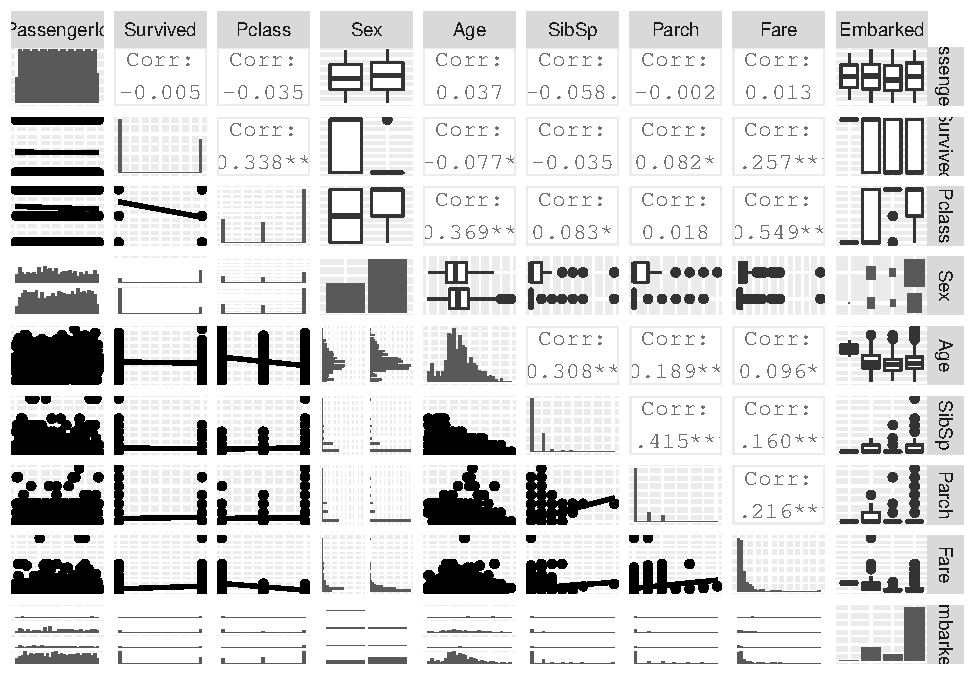
\includegraphics{m2851_PRA2_aruizplaza_rcotillas_files/figure-latex/unnamed-chunk-2-1.pdf}

Aunque con la función ggpairs aporta mucha información acerca de las
distribuciones y correlacciones de las variables, los gráficos aportados
son excesivamente pequeños y no se entienden bien. Para visualizar un
poco mejor dichos gráficos se recomienda, si está visualizando desde
RStudio, usar la opción ver en nueva ventana, que permite ver la matríz
de gráficos, más grande.

Queriamos aprovechar tambien la potencia y los concimientos que tenemos
de python, y hemos estimado el usar ambos lenguajes en esta practica
usando la libreria Reticulate.

\begin{Shaded}
\begin{Highlighting}[]
\CommentTok{# Transfomamos el dataset de R a un dataframe de Pandas (python) }
\NormalTok{pdTrain <-}\StringTok{ }\KeywordTok{r_to_py}\NormalTok{(dfTrain)}
\end{Highlighting}
\end{Shaded}

Se observan los tipos de variables que del dataframe transformado:

\begin{Shaded}
\begin{Highlighting}[]
\NormalTok{r.pdTrain.info()}
\end{Highlighting}
\end{Shaded}

\begin{verbatim}
## <class 'pandas.core.frame.DataFrame'>
## RangeIndex: 891 entries, 0 to 890
## Data columns (total 12 columns):
##  #   Column       Non-Null Count  Dtype  
## ---  ------       --------------  -----  
##  0   PassengerId  891 non-null    int32  
##  1   Survived     891 non-null    int32  
##  2   Pclass       891 non-null    int32  
##  3   Name         891 non-null    object 
##  4   Sex          891 non-null    object 
##  5   Age          714 non-null    float64
##  6   SibSp        891 non-null    int32  
##  7   Parch        891 non-null    int32  
##  8   Ticket       891 non-null    object 
##  9   Fare         891 non-null    float64
##  10  Cabin        891 non-null    object 
##  11  Embarked     891 non-null    object 
## dtypes: float64(2), int32(5), object(5)
## memory usage: 66.3+ KB
\end{verbatim}

\textbf{A continuación definimos, en Python, dos funciones que nos
permitiran generar las diferentes visualizaciones de Distribuciones de
datos e Histogramas que deseamos utilizar:}

\begin{Shaded}
\begin{Highlighting}[]
\CommentTok{#test["Pclass"].value_counts().sort_index().plot(kind="bar", colormap='Paired')}
\KeywordTok{def}\NormalTok{ viewDist(x, data, hue}\OperatorTok{=}\VariableTok{None}\NormalTok{):}
\NormalTok{    fig, axs }\OperatorTok{=}\NormalTok{ plt.subplots(ncols}\OperatorTok{=}\DecValTok{2}\NormalTok{, constrained_layout}\OperatorTok{=}\VariableTok{True}\NormalTok{, figsize}\OperatorTok{=}\NormalTok{(}\DecValTok{10}\NormalTok{,}\DecValTok{4}\NormalTok{))}

\NormalTok{    sns.countplot(x}\OperatorTok{=}\NormalTok{x, hue}\OperatorTok{=}\NormalTok{hue, data}\OperatorTok{=}\NormalTok{data, ax}\OperatorTok{=}\NormalTok{axs[}\DecValTok{0}\NormalTok{]).}\BuiltInTok{set}\NormalTok{(title}\OperatorTok{=}\StringTok{'Train'}\NormalTok{)}
\NormalTok{    sns.countplot(x}\OperatorTok{=}\NormalTok{x, hue}\OperatorTok{=}\StringTok{'Survived'}\NormalTok{, data}\OperatorTok{=}\NormalTok{data, ax}\OperatorTok{=}\NormalTok{axs[}\DecValTok{1}\NormalTok{]).}\BuiltInTok{set}\NormalTok{(title}\OperatorTok{=}\StringTok{'Train with Survived'}\NormalTok{)}
\NormalTok{    plt.show()}

\KeywordTok{def}\NormalTok{ viewHist(x, data, hue}\OperatorTok{=}\VariableTok{None}\NormalTok{):}
\NormalTok{    fig, axs }\OperatorTok{=}\NormalTok{ plt.subplots(ncols}\OperatorTok{=}\DecValTok{2}\NormalTok{, constrained_layout}\OperatorTok{=}\VariableTok{True}\NormalTok{,figsize}\OperatorTok{=}\NormalTok{(}\DecValTok{15}\NormalTok{,}\DecValTok{4}\NormalTok{))}
    
\NormalTok{    sns.histplot(data[x], ax}\OperatorTok{=}\NormalTok{axs[}\DecValTok{0}\NormalTok{]).}\BuiltInTok{set}\NormalTok{(title}\OperatorTok{=}\StringTok{'Train Hist'}\NormalTok{)}
\NormalTok{    sns.boxplot(x}\OperatorTok{=}\NormalTok{data[x], ax}\OperatorTok{=}\NormalTok{axs[}\DecValTok{1}\NormalTok{]).}\BuiltInTok{set}\NormalTok{(title}\OperatorTok{=}\StringTok{'Train Box'}\NormalTok{)}
\NormalTok{    plt.show()}
\end{Highlighting}
\end{Shaded}

Se observa la distribución del campo PClass, tanto de marera aislada,
como relacionada con la variable que se quiere predecir (Survived).

\begin{Shaded}
\begin{Highlighting}[]
\NormalTok{viewDist(}\StringTok{"Pclass"}\NormalTok{, r.pdTrain)}
\end{Highlighting}
\end{Shaded}

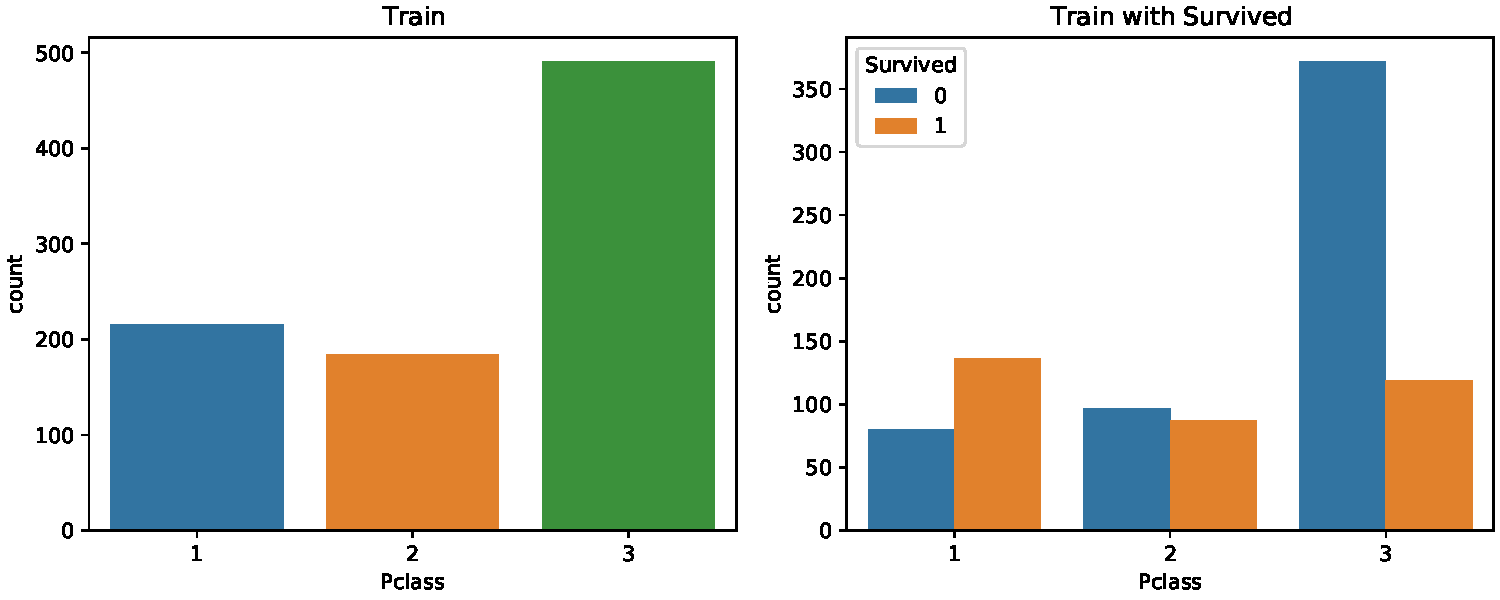
\includegraphics{m2851_PRA2_aruizplaza_rcotillas_files/figure-latex/unnamed-chunk-6-1.pdf}

Aquí podemos ver, tal y como se comentó al analizar los resultados de
sumary y describe, que la mayoría de pasajeros se ubican en 3a clase.
También podemos observar que el porcentaje de supervivientes en la 3a
clase, es mucho menor que en primera y segunda.

\textbf{Se observa la distribución del campo Sex, tanto de marera
aislada, como relacionada con la variable que se quiere predecir
(Survived).}

\begin{Shaded}
\begin{Highlighting}[]
\NormalTok{viewDist(}\StringTok{"Sex"}\NormalTok{, r.pdTrain)}
\end{Highlighting}
\end{Shaded}

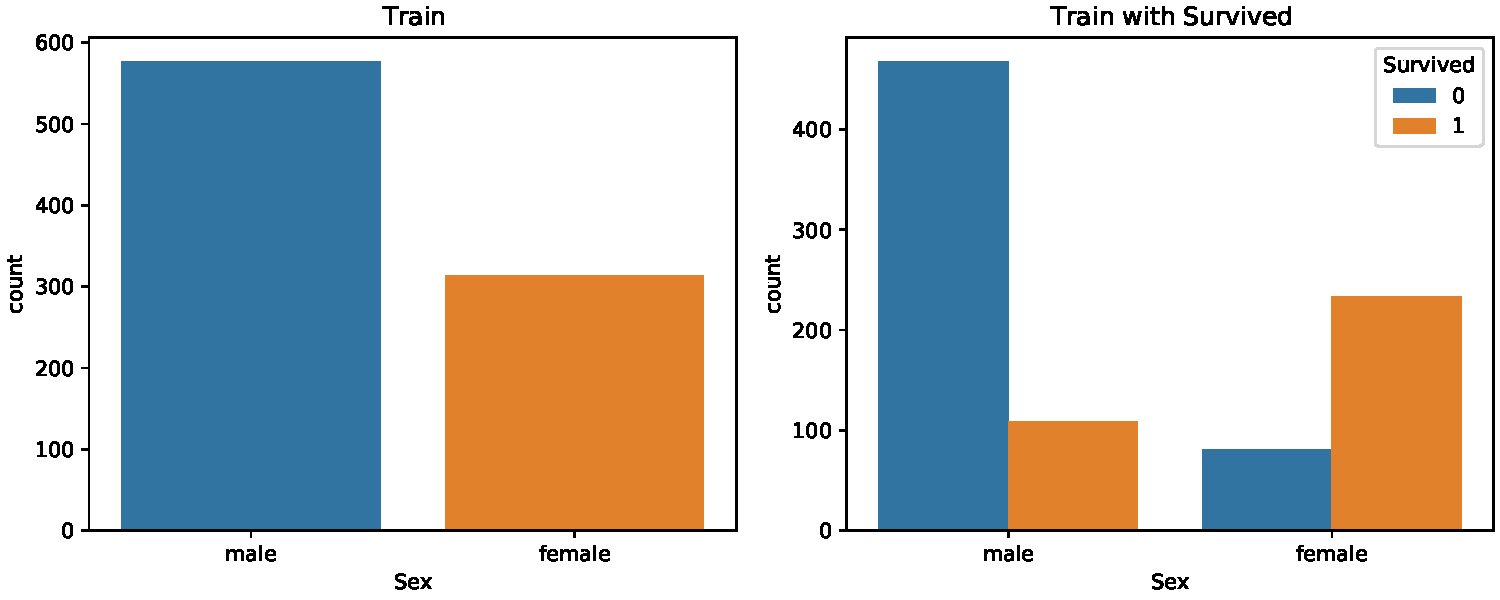
\includegraphics{m2851_PRA2_aruizplaza_rcotillas_files/figure-latex/unnamed-chunk-7-1.pdf}

Si observamos los gráficos anteriores, vemos que a pesar de que
embarcaron casi el doble de hombres que mujeres, el número de
supervivientes masculinos fue menos de la mitad que el número de
mujeres.

\textbf{A continuación, se observa el histograma sobre el campo Age, y
además, un boxplot que nos permite localizar posibles candidatos a
outlier.}

\begin{Shaded}
\begin{Highlighting}[]
\NormalTok{viewHist(}\StringTok{"Age"}\NormalTok{, r.pdTrain)}
\end{Highlighting}
\end{Shaded}

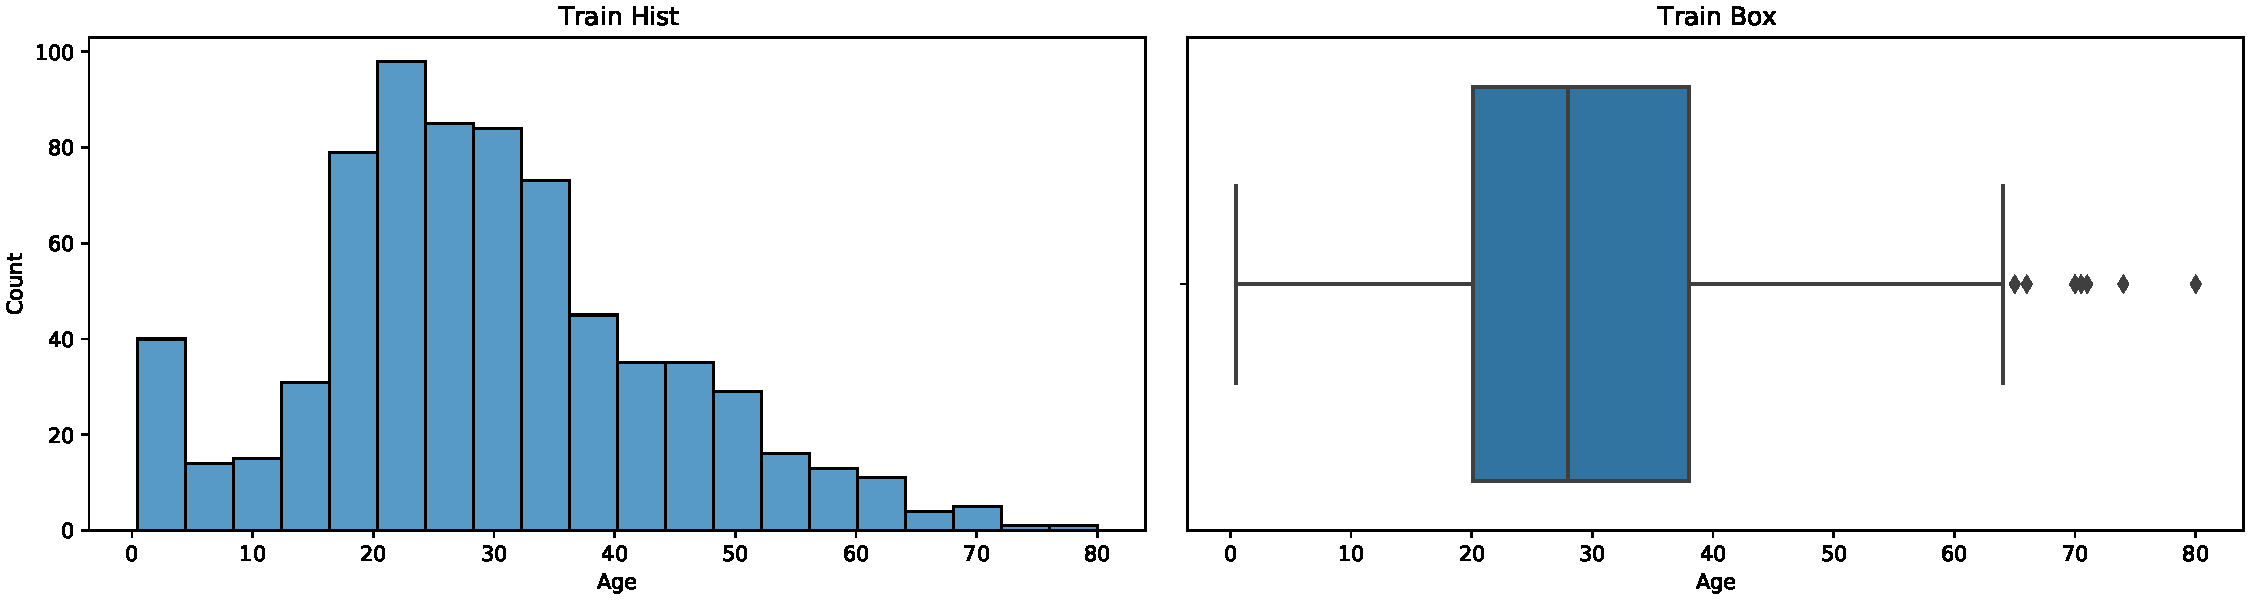
\includegraphics{m2851_PRA2_aruizplaza_rcotillas_files/figure-latex/unnamed-chunk-8-1.pdf}

Si nos fijamos en el boxplot basado en la variable Age, vemos que la
gran mayoría del pasaje entaba en la franja entre 20 y 40 años, y no
abundaban personas con más de 65 años.

\textbf{A continuación, se observa la distribución del campo SibSp,
tanto de marera aislada, como relacionada con la variable que se quiere
predecir (Survived).}

\begin{Shaded}
\begin{Highlighting}[]
\NormalTok{viewDist(}\StringTok{"SibSp"}\NormalTok{, r.pdTrain)}
\end{Highlighting}
\end{Shaded}

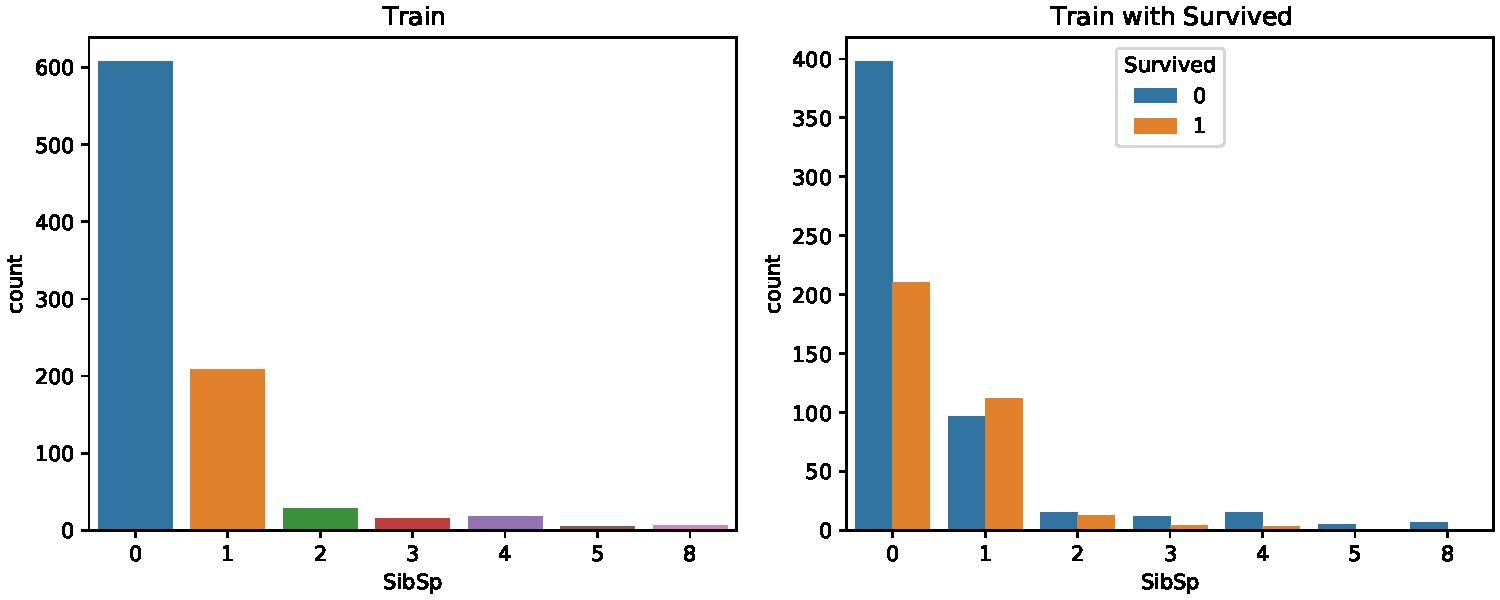
\includegraphics{m2851_PRA2_aruizplaza_rcotillas_files/figure-latex/unnamed-chunk-9-1.pdf}

Si nos atenemos a la distribución de la variable SibSp, si los datos son
correctos, podríamos decir que la mayoría de pasajeros viajaban sin
hermanos ni pareja.

\textbf{A continuación, se observa la distribución del campo Parch,
tanto de marera aislada, como relacionada con la variable que se quiere
predecir (Survived).}

\begin{Shaded}
\begin{Highlighting}[]
\NormalTok{viewDist(}\StringTok{"Parch"}\NormalTok{, r.pdTrain)}
\end{Highlighting}
\end{Shaded}

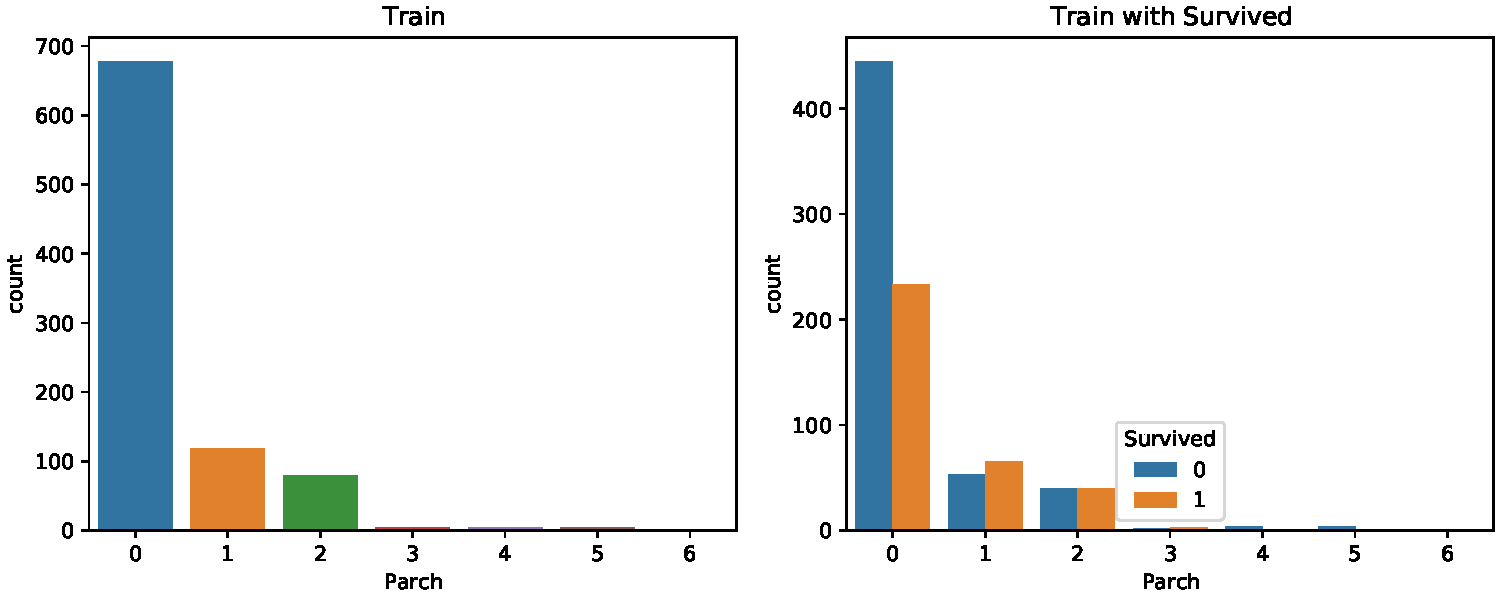
\includegraphics{m2851_PRA2_aruizplaza_rcotillas_files/figure-latex/unnamed-chunk-10-1.pdf}

En cuanto a la variable Parch que nos indica si el pasajero viajaba con
padres o hijos, si observamos la distribución de los valores, podríamos
decir que la mayoría de pasajeros viajaban sin padres ni hijos.

\begin{Shaded}
\begin{Highlighting}[]
\NormalTok{viewHist(}\StringTok{"Fare"}\NormalTok{, r.pdTrain)}
\end{Highlighting}
\end{Shaded}

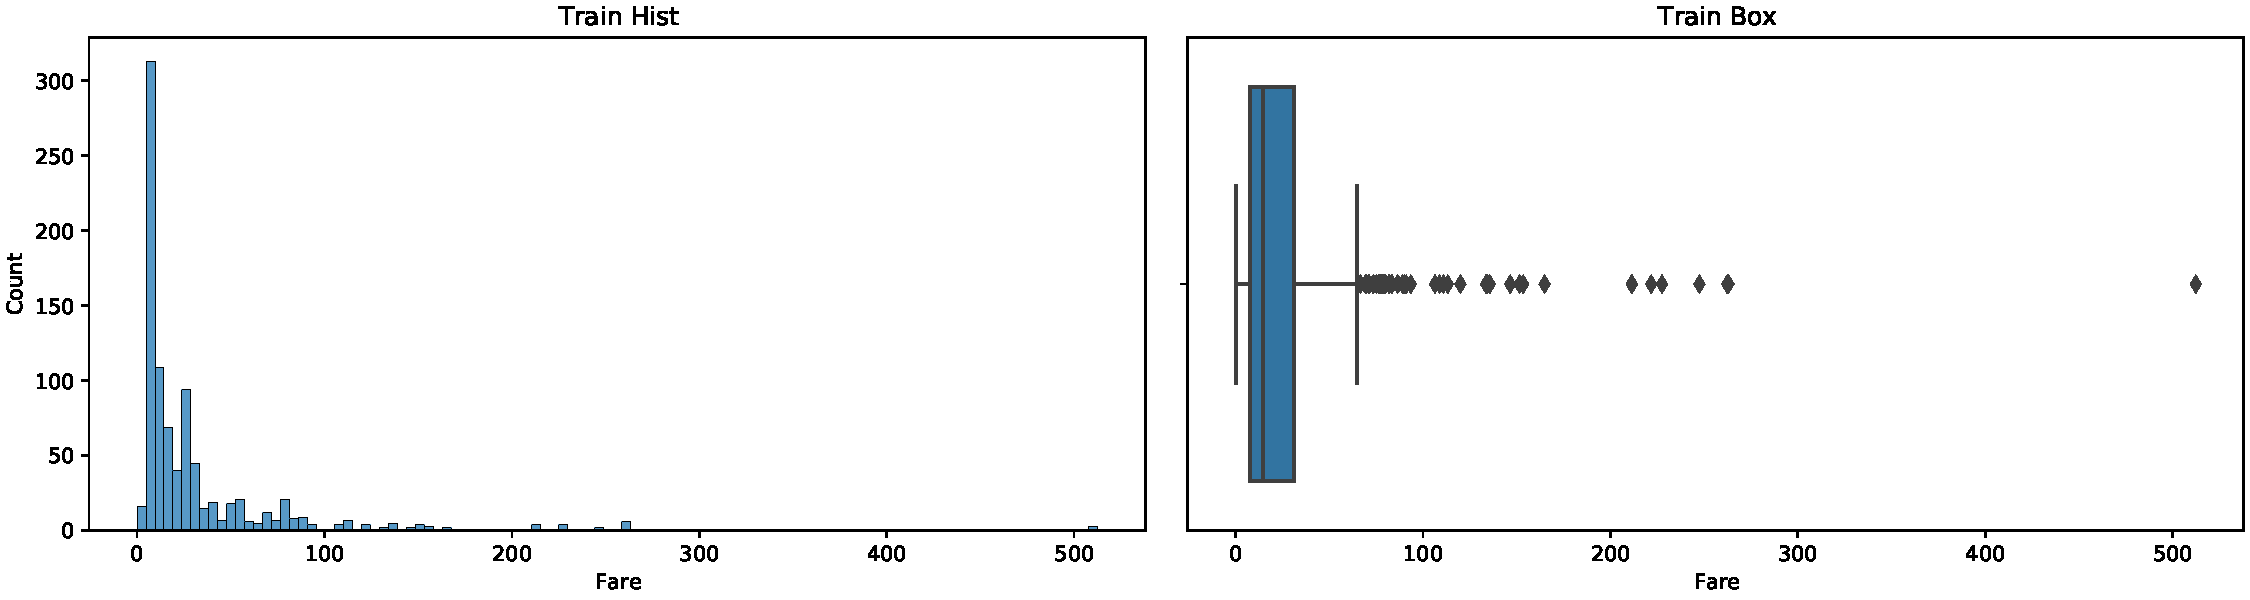
\includegraphics{m2851_PRA2_aruizplaza_rcotillas_files/figure-latex/unnamed-chunk-11-1.pdf}

Si observamos el histograma y el boxplot realizados sobre la variable
Fare, podríamos considerar como outliers aquellas tarifas que superen
las 60 Libras, sin embargo, este tema se aborda en el apartado de
outliers.

\begin{Shaded}
\begin{Highlighting}[]
\NormalTok{viewDist(}\StringTok{"Embarked"}\NormalTok{, r.pdTrain)}
\end{Highlighting}
\end{Shaded}

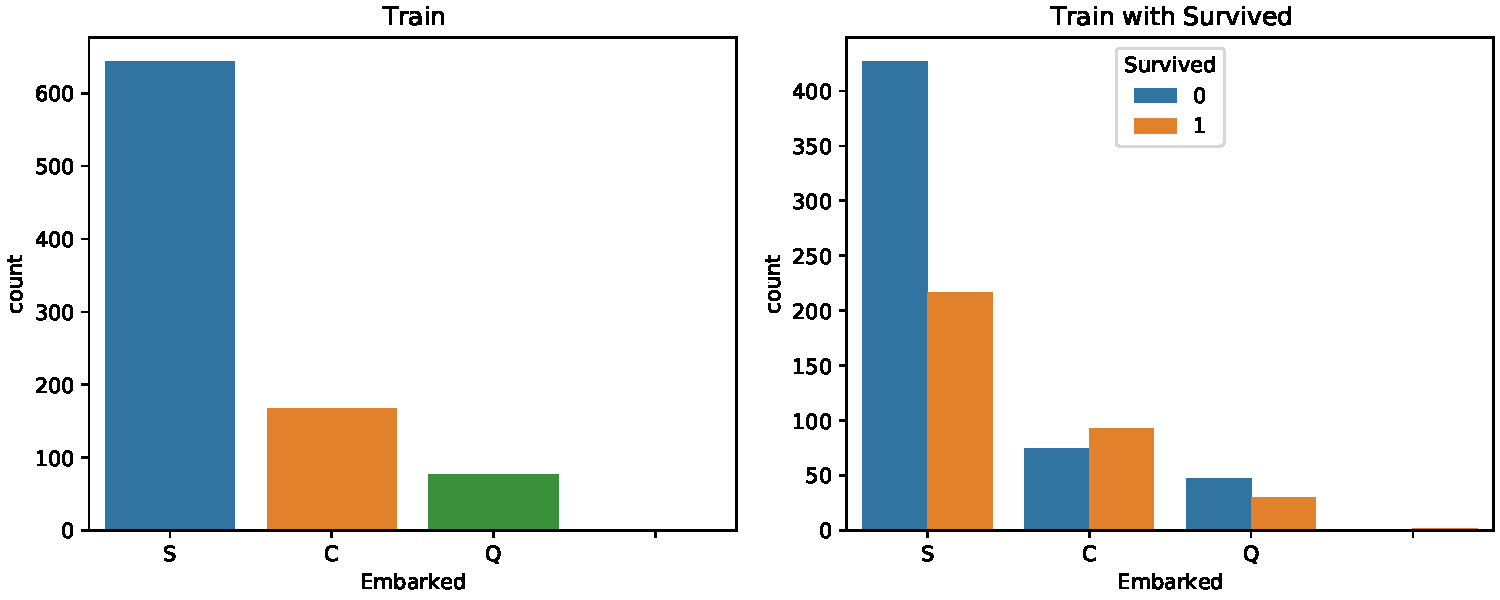
\includegraphics{m2851_PRA2_aruizplaza_rcotillas_files/figure-latex/unnamed-chunk-12-1.pdf}

Podemos ver que la mayoría de los pasajeros embarcaron en
Southampton(S), sin embargo, el indice de supervivientes es mayor entre
los que embarcaron en Cherbourg(C) o Queenstown (Q).

\begin{Shaded}
\begin{Highlighting}[]
\NormalTok{correlation_mat }\OperatorTok{=}\NormalTok{ r.dfTrain.corr()}
\NormalTok{sns.heatmap(correlation_mat, annot }\OperatorTok{=} \VariableTok{True}\NormalTok{)}
\NormalTok{plt.show()}
\end{Highlighting}
\end{Shaded}

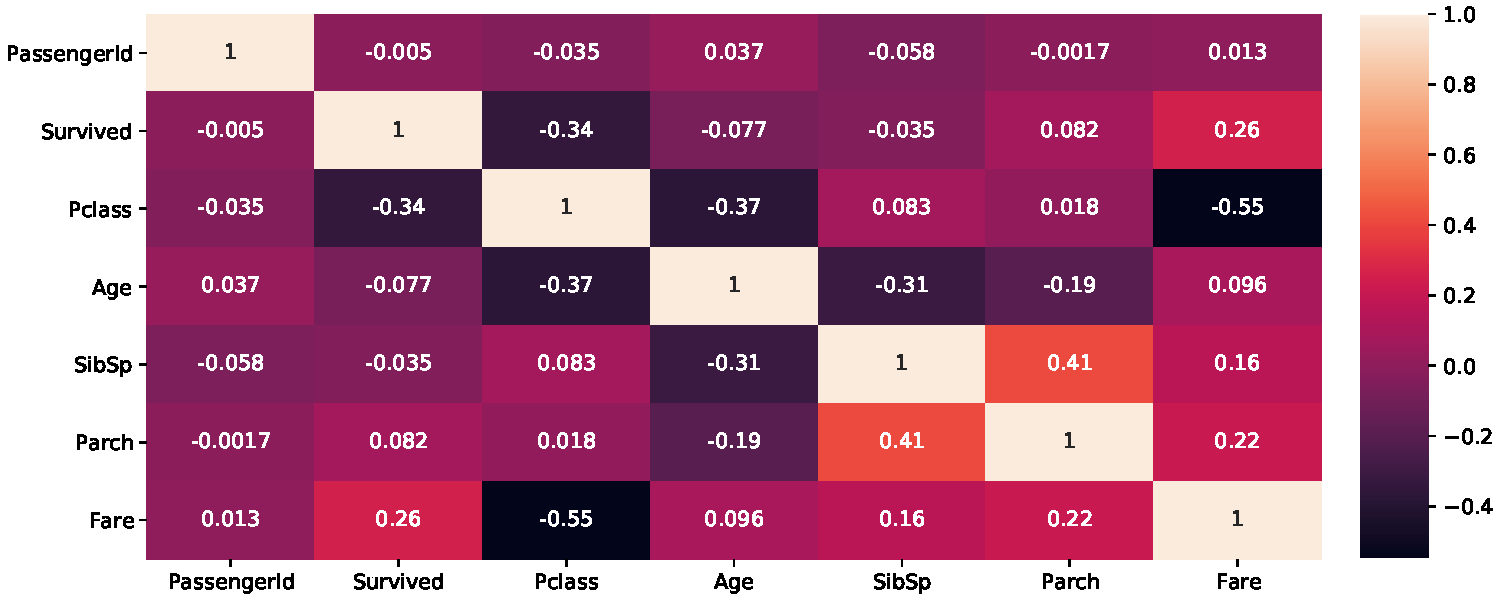
\includegraphics{m2851_PRA2_aruizplaza_rcotillas_files/figure-latex/unnamed-chunk-13-1.pdf}

\hypertarget{limpieza-de-los-datos.}{%
\section{.- Limpieza de los datos.}\label{limpieza-de-los-datos.}}

Preparación de datos (Según las necesidades del modelo a aplicar en cada
caso)

\hypertarget{los-datos-contienen-ceros-o-elementos-vacuxedos-cuxf3mo-gestionaruxedas-cada-uno-de-estos-casos}{%
\subsection{.- ¿Los datos contienen ceros o elementos vacíos? ¿Cómo
gestionarías cada uno de estos
casos?}\label{los-datos-contienen-ceros-o-elementos-vacuxedos-cuxf3mo-gestionaruxedas-cada-uno-de-estos-casos}}

\textbf{Observamos los valores nulos de las diferentes variables:}

\begin{Shaded}
\begin{Highlighting}[]
\CommentTok{# Mediante observación directa del fichero csv y las información obtenida en el estudio ya realizado, se observa que los campos Cabin y Embarked contienen valores desconocidos representados con "".}

\CommentTok{# Número de valores "" contenidos por la variable Cabin}
\KeywordTok{cat}\NormalTok{(}\StringTok{"Numero de valores nulos en Cavin:"}\NormalTok{, }\KeywordTok{NROW}\NormalTok{(dfTrain}\OperatorTok{$}\NormalTok{Cabin[dfTrain}\OperatorTok{$}\NormalTok{Cabin }\OperatorTok{==}\StringTok{ ""}\NormalTok{]))}
\end{Highlighting}
\end{Shaded}

\begin{verbatim}
## Numero de valores nulos en Cavin: 687
\end{verbatim}

\begin{Shaded}
\begin{Highlighting}[]
\CommentTok{# Valores únicos para Embarked}
\KeywordTok{cat}\NormalTok{(}\StringTok{"Valores únicos para Embarked:"}\NormalTok{)}
\end{Highlighting}
\end{Shaded}

\begin{verbatim}
## Valores únicos para Embarked:
\end{verbatim}

\begin{Shaded}
\begin{Highlighting}[]
\KeywordTok{unique}\NormalTok{(dfTrain}\OperatorTok{$}\NormalTok{Embarked)}
\end{Highlighting}
\end{Shaded}

\begin{verbatim}
## [1] "S" "C" "Q" ""
\end{verbatim}

\begin{Shaded}
\begin{Highlighting}[]
\CommentTok{# Valores nulos en enbarked}
\KeywordTok{cat}\NormalTok{(}\StringTok{"Numero de valores nulos para Embarked: "}\NormalTok{,}\KeywordTok{NROW}\NormalTok{(dfTrain}\OperatorTok{$}\NormalTok{Embarked[dfTrain}\OperatorTok{$}\NormalTok{Embarked }\OperatorTok{==}\StringTok{ ""}\NormalTok{]))}
\end{Highlighting}
\end{Shaded}

\begin{verbatim}
## Numero de valores nulos para Embarked:  2
\end{verbatim}

\begin{Shaded}
\begin{Highlighting}[]
\CommentTok{#Recodificamos como valores desconocidos aquellos valores == "" en los campos mencionados anteriormente}
\NormalTok{dfTrain}\OperatorTok{$}\NormalTok{Cabin[dfTrain}\OperatorTok{$}\NormalTok{Cabin }\OperatorTok{==}\StringTok{ ""}\NormalTok{] <-}\StringTok{ }\OtherTok{NA}
\NormalTok{dfTrain}\OperatorTok{$}\NormalTok{Embarked[dfTrain}\OperatorTok{$}\NormalTok{Embarked }\OperatorTok{==}\StringTok{ ""}\NormalTok{] <-}\StringTok{ }\OtherTok{NA}

\CommentTok{# Estadísticas de valores vacíos}
\KeywordTok{colSums}\NormalTok{(}\KeywordTok{is.na}\NormalTok{(dfTrain))}
\end{Highlighting}
\end{Shaded}

\begin{verbatim}
## PassengerId    Survived      Pclass        Name         Sex         Age 
##           0           0           0           0           0         177 
##       SibSp       Parch      Ticket        Fare       Cabin    Embarked 
##           0           0           0           0         687           2
\end{verbatim}

A continuación se estudia la opción de reemplazar los valores nulos de
la variable Cabin por algo más útil. Según parece, la letra que precede
al número que identifica una cabina, indica la sección donde se ubica la
misma, generamos, y factorizamos, una nueva variable ``Sector'' a partir
de la letra inicial de la cabina. Los valores nulos se reemplazan por el
valor ``0''.

\begin{Shaded}
\begin{Highlighting}[]
\NormalTok{dfTrain}\OperatorTok{$}\NormalTok{Sector[}\OperatorTok{!}\KeywordTok{is.na}\NormalTok{(dfTrain}\OperatorTok{$}\NormalTok{Cabin)] <-}\StringTok{ }\KeywordTok{as.factor}\NormalTok{(}\KeywordTok{substr}\NormalTok{(dfTrain[}\OperatorTok{!}\KeywordTok{is.na}\NormalTok{(dfTrain}\OperatorTok{$}\NormalTok{Cabin),]}\OperatorTok{$}\NormalTok{Cabin,}\DecValTok{1}\NormalTok{,}\DecValTok{1}\NormalTok{))}
\NormalTok{dfTrain}\OperatorTok{$}\NormalTok{Sector[}\KeywordTok{is.na}\NormalTok{(dfTrain}\OperatorTok{$}\NormalTok{Cabin)] <-}\StringTok{ "0"}
\CommentTok{#dfTrain$Sector}
\end{Highlighting}
\end{Shaded}

A continuación, se observa la distribución de la nueva variable
(Sector), tanto de marera aislada, como relacionada con la variable que
se quiere predecir (Survived).

\begin{Shaded}
\begin{Highlighting}[]
\NormalTok{viewDist(}\StringTok{"Sector"}\NormalTok{, r.dfTrain)}
\end{Highlighting}
\end{Shaded}

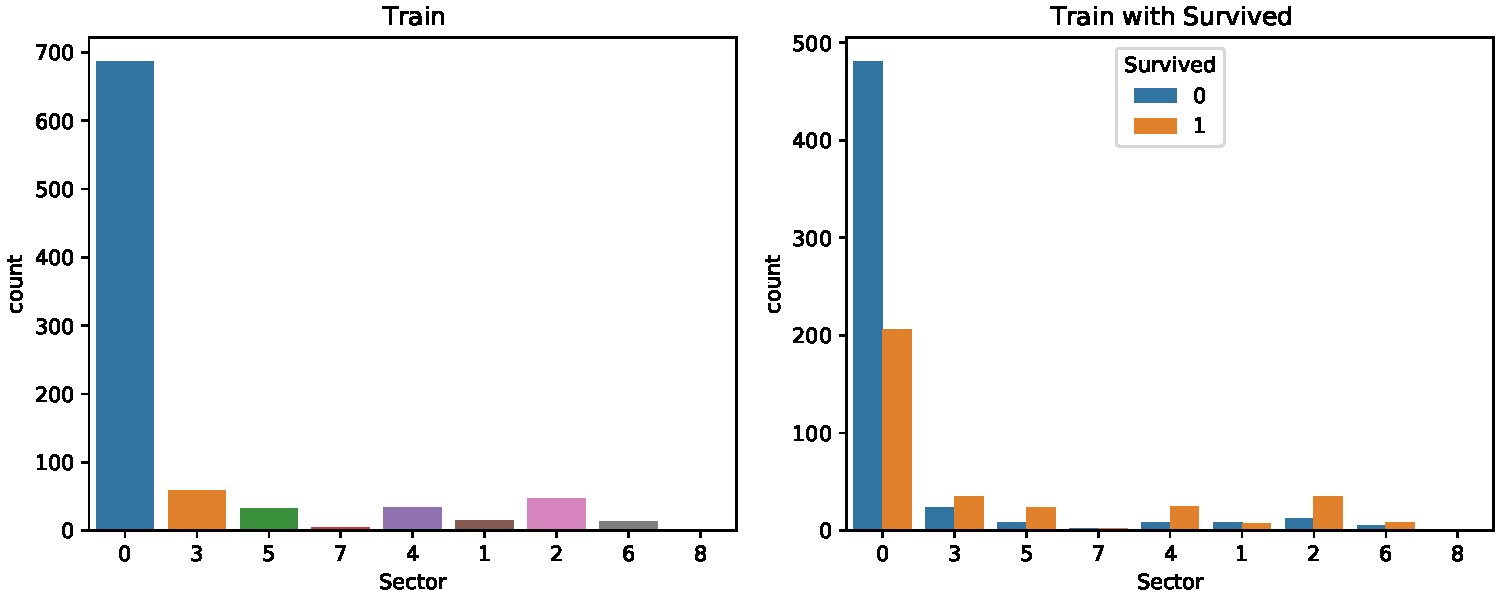
\includegraphics{m2851_PRA2_aruizplaza_rcotillas_files/figure-latex/unnamed-chunk-18-1.pdf}

\begin{Shaded}
\begin{Highlighting}[]
\CommentTok{# Creamos nuevo data frame sobre el que trabajaremos para obtener todas las variables de tipo numérico, factorizando las variables categóricas. }
\NormalTok{dfTrain_cat <-}\StringTok{ }\NormalTok{dfTrain}

\CommentTok{# Verificamos la estructura del juego de datos y factorizamos las variables categóricas (Sex, Embarked y Sector(obtenida a partir de Cabin))}
\KeywordTok{str}\NormalTok{(dfTrain_cat)}
\end{Highlighting}
\end{Shaded}

\begin{verbatim}
## 'data.frame':    891 obs. of  13 variables:
##  $ PassengerId: int  1 2 3 4 5 6 7 8 9 10 ...
##  $ Survived   : int  0 1 1 1 0 0 0 0 1 1 ...
##  $ Pclass     : int  3 1 3 1 3 3 1 3 3 2 ...
##  $ Name       : chr  "Braund, Mr. Owen Harris" "Cumings, Mrs. John Bradley (Florence Briggs Thayer)" "Heikkinen, Miss. Laina" "Futrelle, Mrs. Jacques Heath (Lily May Peel)" ...
##  $ Sex        : chr  "male" "female" "female" "female" ...
##  $ Age        : num  22 38 26 35 35 NA 54 2 27 14 ...
##  $ SibSp      : int  1 1 0 1 0 0 0 3 0 1 ...
##  $ Parch      : int  0 0 0 0 0 0 0 1 2 0 ...
##  $ Ticket     : chr  "A/5 21171" "PC 17599" "STON/O2. 3101282" "113803" ...
##  $ Fare       : num  7.25 71.28 7.92 53.1 8.05 ...
##  $ Cabin      : chr  NA "C85" NA "C123" ...
##  $ Embarked   : chr  "S" "C" "S" "S" ...
##  $ Sector     : chr  "0" "3" "0" "3" ...
\end{verbatim}

\begin{Shaded}
\begin{Highlighting}[]
\CommentTok{# Discretizamos la edad creando 5 rangos de edades: Bebé(0-3], Infante(3-13], joven(13-29), Adulto(29,60], Anciano(60,100]}
\NormalTok{dfTrain_cat}\OperatorTok{$}\NormalTok{Age <-}\StringTok{ }\KeywordTok{cut}\NormalTok{(dfTrain_cat}\OperatorTok{$}\NormalTok{Age, }\KeywordTok{c}\NormalTok{(}\DecValTok{0}\NormalTok{,}\DecValTok{3}\NormalTok{,}\DecValTok{13}\NormalTok{,}\DecValTok{29}\NormalTok{,}\DecValTok{60}\NormalTok{,}\DecValTok{100}\NormalTok{), }\DataTypeTok{labels=}\KeywordTok{c}\NormalTok{(}\DecValTok{1}\OperatorTok{:}\DecValTok{5}\NormalTok{))}


\CommentTok{# Eliminamos del dataset las variables Ticket y Cabin}
\NormalTok{dfTrain_cat <-}\StringTok{ }\NormalTok{dfTrain_cat[}\OperatorTok{-}\KeywordTok{c}\NormalTok{(}\DecValTok{9}\NormalTok{,}\DecValTok{11}\NormalTok{)]}

\CommentTok{# Creamos nuevo data frame sobre el que trabajaremos para obtener todas las variables de tipo numérico, factorizando las variables categóricas. }

\NormalTok{dfTrain_cat}\OperatorTok{$}\NormalTok{Sex <-}\StringTok{ }\KeywordTok{as.factor}\NormalTok{(dfTrain_cat}\OperatorTok{$}\NormalTok{Sex)}
\NormalTok{dfTrain_cat}\OperatorTok{$}\NormalTok{Embarked <-}\StringTok{ }\KeywordTok{as.factor}\NormalTok{(dfTrain_cat}\OperatorTok{$}\NormalTok{Embarked)}
\NormalTok{dfTrain_cat}\OperatorTok{$}\NormalTok{Age <-}\StringTok{ }\KeywordTok{as.factor}\NormalTok{(dfTrain_cat}\OperatorTok{$}\NormalTok{Age)}
\NormalTok{dfTrain_cat}\OperatorTok{$}\NormalTok{Pclass <-}\StringTok{ }\KeywordTok{as.factor}\NormalTok{(dfTrain_cat}\OperatorTok{$}\NormalTok{Pclass)}
\NormalTok{dfTrain_cat}\OperatorTok{$}\NormalTok{SibSp <-}\StringTok{ }\KeywordTok{as.factor}\NormalTok{(dfTrain_cat}\OperatorTok{$}\NormalTok{SibSp)}
\NormalTok{dfTrain_cat}\OperatorTok{$}\NormalTok{Parch <-}\StringTok{ }\KeywordTok{as.factor}\NormalTok{(dfTrain_cat}\OperatorTok{$}\NormalTok{Parch)}
\NormalTok{dfTrain_cat}\OperatorTok{$}\NormalTok{Sector<-}\StringTok{ }\KeywordTok{as.factor}\NormalTok{(dfTrain_cat}\OperatorTok{$}\NormalTok{Sector)}

\CommentTok{# Eliminamos del dataset la variable Name}
\NormalTok{dfTrain_cat <-}\StringTok{ }\NormalTok{dfTrain_cat[}\OperatorTok{-}\DecValTok{4}\NormalTok{]}

\CommentTok{# Eliminamos del dataset la variable PassengerId}
\NormalTok{dfTrain_cat <-}\StringTok{ }\NormalTok{dfTrain_cat[}\OperatorTok{-}\DecValTok{1}\NormalTok{]}


\KeywordTok{str}\NormalTok{(dfTrain_cat)}
\end{Highlighting}
\end{Shaded}

\begin{verbatim}
## 'data.frame':    891 obs. of  9 variables:
##  $ Survived: int  0 1 1 1 0 0 0 0 1 1 ...
##  $ Pclass  : Factor w/ 3 levels "1","2","3": 3 1 3 1 3 3 1 3 3 2 ...
##  $ Sex     : Factor w/ 2 levels "female","male": 2 1 1 1 2 2 2 2 1 1 ...
##  $ Age     : Factor w/ 5 levels "1","2","3","4",..: 3 4 3 4 4 NA 4 1 3 3 ...
##  $ SibSp   : Factor w/ 7 levels "0","1","2","3",..: 2 2 1 2 1 1 1 4 1 2 ...
##  $ Parch   : Factor w/ 7 levels "0","1","2","3",..: 1 1 1 1 1 1 1 2 3 1 ...
##  $ Fare    : num  7.25 71.28 7.92 53.1 8.05 ...
##  $ Embarked: Factor w/ 3 levels "C","Q","S": 3 1 3 3 3 2 3 3 3 1 ...
##  $ Sector  : Factor w/ 9 levels "0","1","2","3",..: 1 4 1 4 1 1 6 1 1 1 ...
\end{verbatim}

Usamos la funcion kNN (vecinos mas cercanos para la imputacion de los
valores nulos en las variables. Nuestra primera opcion fue usar la media
sin embargo pensamos que usar un método de imputacion basado en la
similitud seria más correcto.

\begin{Shaded}
\begin{Highlighting}[]
\NormalTok{dfTrain_cat}\OperatorTok{$}\NormalTok{Embarked <-}\StringTok{ }\KeywordTok{kNN}\NormalTok{(dfTrain_cat)}\OperatorTok{$}\NormalTok{Embarked}
\KeywordTok{colSums}\NormalTok{(}\KeywordTok{is.na}\NormalTok{(dfTrain_cat))}
\end{Highlighting}
\end{Shaded}

\begin{verbatim}
## Survived   Pclass      Sex      Age    SibSp    Parch     Fare Embarked 
##        0        0        0      177        0        0        0        0 
##   Sector 
##        0
\end{verbatim}

Una vez se tienen el campo edad categorizado, volvemos a aplicar el
modelo a ver si esta vez es viable su uso. (Se ha ejecutado varias veces
para ver los p-valores de las variables y descartar aquellas que no
tengan significancia). Pero antes de ello visualizamos como esta
distribuida la variable Age una vez categorizada y su relaccion con la
variable survived.

\begin{Shaded}
\begin{Highlighting}[]
\NormalTok{viewDist(}\StringTok{"Age"}\NormalTok{, r.dfTrain_cat)}
\end{Highlighting}
\end{Shaded}

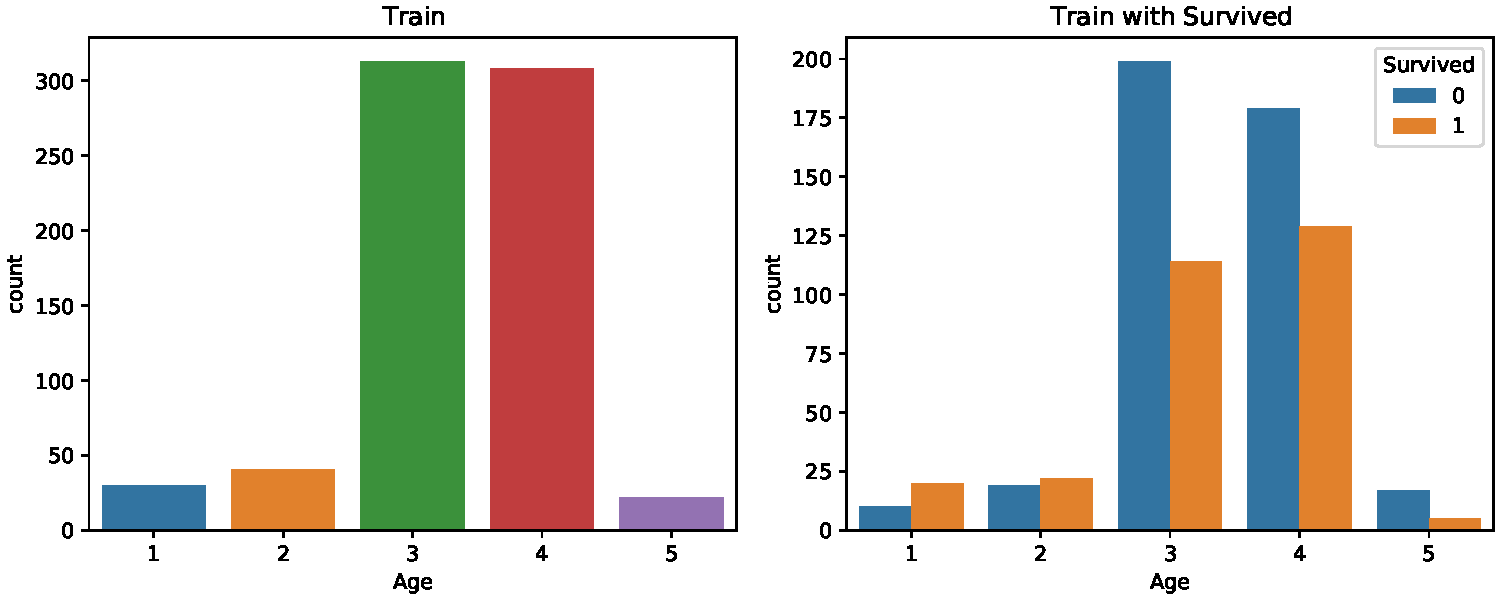
\includegraphics{m2851_PRA2_aruizplaza_rcotillas_files/figure-latex/unnamed-chunk-21-1.pdf}
Observando la gráfica podemos entender que si eras bebe tenias muchas
probabilidades de sobrevivir y los niños un poco más del 50\%. Si eras
un anciano las posibilidades eran bajas y para el resto de rango de
edades estaba parejo, por lo que se podría categorizar en la misma
franja (quedando los siguientes rangos de edad: bebes, niños, adultos y
ancianos).

\begin{Shaded}
\begin{Highlighting}[]
\NormalTok{dfTrain_cat_age <-}\StringTok{ }\NormalTok{dfTrain_cat[}\OperatorTok{!}\KeywordTok{is.na}\NormalTok{(dfTrain_cat}\OperatorTok{$}\NormalTok{Age),]}

\NormalTok{model_age_cat <-}\StringTok{ }\KeywordTok{lm}\NormalTok{(}\KeywordTok{as.numeric}\NormalTok{(Age)}\OperatorTok{~}\KeywordTok{as.numeric}\NormalTok{(Pclass) }\OperatorTok{+}\StringTok{ }\KeywordTok{as.numeric}\NormalTok{(SibSp) }\OperatorTok{+}\StringTok{ }\KeywordTok{as.numeric}\NormalTok{(Parch), }\DataTypeTok{data =}\NormalTok{ dfTrain_cat_age)}
\KeywordTok{summary}\NormalTok{(model_age_cat)}
\end{Highlighting}
\end{Shaded}

\begin{verbatim}
## 
## Call:
## lm(formula = as.numeric(Age) ~ as.numeric(Pclass) + as.numeric(SibSp) + 
##     as.numeric(Parch), data = dfTrain_cat_age)
## 
## Residuals:
##      Min       1Q   Median       3Q      Max 
## -2.36670 -0.33002  0.04951  0.50968  1.88055 
## 
## Coefficients:
##                    Estimate Std. Error t value Pr(>|t|)    
## (Intercept)         4.51930    0.09105  49.634  < 2e-16 ***
## as.numeric(Pclass) -0.26992    0.03207  -8.416  < 2e-16 ***
## as.numeric(SibSp)  -0.25590    0.03130  -8.176 1.35e-15 ***
## as.numeric(Parch)  -0.12362    0.03404  -3.632 0.000302 ***
## ---
## Signif. codes:  0 '***' 0.001 '**' 0.01 '*' 0.05 '.' 0.1 ' ' 1
## 
## Residual standard error: 0.7162 on 710 degrees of freedom
## Multiple R-squared:  0.2231, Adjusted R-squared:  0.2198 
## F-statistic: 67.96 on 3 and 710 DF,  p-value: < 2.2e-16
\end{verbatim}

Se observa qué el Ajusted R-squared es bastante bajo (0,2198). Hay que
tener en cuenta que el dataset se ha quedado desbalancedo, ya que hay
muchos registros del tipo 3 y 4, pocos del tipo 1, 2 y 5.

\textbf{Probamos otro modelo, tratando de conseguir una mayor
precisión.}

\begin{Shaded}
\begin{Highlighting}[]
\CommentTok{## 80% of the sample size}
\NormalTok{smp_size <-}\StringTok{ }\KeywordTok{floor}\NormalTok{(}\FloatTok{0.80} \OperatorTok{*}\StringTok{ }\KeywordTok{nrow}\NormalTok{(dfTrain_cat_age))}

\CommentTok{## set the seed to make your partition reproducible}
\KeywordTok{set.seed}\NormalTok{(}\DecValTok{123}\NormalTok{)}
\NormalTok{train_ind <-}\StringTok{ }\KeywordTok{sample}\NormalTok{(}\KeywordTok{seq_len}\NormalTok{(}\KeywordTok{nrow}\NormalTok{(dfTrain_cat_age)), }\DataTypeTok{size =}\NormalTok{ smp_size)}

\NormalTok{train <-}\StringTok{ }\NormalTok{dfTrain_cat_age[train_ind, ]}
\NormalTok{test <-}\StringTok{ }\NormalTok{dfTrain_cat_age[}\OperatorTok{-}\NormalTok{train_ind, ]}

\CommentTok{# Usamos Bagging nos permite combinar los resultados de varios modelos de clasificación para conseguir mejores resultados.}
\NormalTok{fit <-}\StringTok{ }\KeywordTok{bagging}\NormalTok{(Age}\OperatorTok{~}\NormalTok{.}\OperatorTok{-}\NormalTok{Sector, }\DataTypeTok{data=}\NormalTok{train)}

\CommentTok{# Predecimos los valores del test}
\NormalTok{pred <-}\StringTok{ }\KeywordTok{predict}\NormalTok{(fit, test)}
\end{Highlighting}
\end{Shaded}

\begin{Shaded}
\begin{Highlighting}[]
\CommentTok{#t = table(pred, test$Age)}
\KeywordTok{confusionMatrix}\NormalTok{(pred, test}\OperatorTok{$}\NormalTok{Age)}
\end{Highlighting}
\end{Shaded}

\begin{verbatim}
## Confusion Matrix and Statistics
## 
##           Reference
## Prediction  1  2  3  4  5
##          1  1  1  0  0  0
##          2  1  2  2  1  0
##          3  1  3 39 39  0
##          4  0  1 18 28  4
##          5  0  0  1  1  0
## 
## Overall Statistics
##                                           
##                Accuracy : 0.4895          
##                  95% CI : (0.4051, 0.5744)
##     No Information Rate : 0.4825          
##     P-Value [Acc > NIR] : 0.4663          
##                                           
##                   Kappa : 0.1267          
##                                           
##  Mcnemar's Test P-Value : NA              
## 
## Statistics by Class:
## 
##                      Class: 1 Class: 2 Class: 3 Class: 4 Class: 5
## Sensitivity          0.333333  0.28571   0.6500   0.4058  0.00000
## Specificity          0.992857  0.97059   0.4819   0.6892  0.98561
## Pos Pred Value       0.500000  0.33333   0.4756   0.5490  0.00000
## Neg Pred Value       0.985816  0.96350   0.6557   0.5543  0.97163
## Prevalence           0.020979  0.04895   0.4196   0.4825  0.02797
## Detection Rate       0.006993  0.01399   0.2727   0.1958  0.00000
## Detection Prevalence 0.013986  0.04196   0.5734   0.3566  0.01399
## Balanced Accuracy    0.663095  0.62815   0.5660   0.5475  0.49281
\end{verbatim}

Si nos fijamos en el accuracy tenemos un modelo muy pobre, uno de los
problemas es que los datos estan poco balanceados, esto se podria
ajustar usando la funcion SMOTE. Sin embargo no vamos a seguir
profundizando, finalmente descartamos el usar un modelo custom para
predecir la edad y lo solucionamos de la misma manera que se ha hecho
con las variables fare y embarked.

\begin{Shaded}
\begin{Highlighting}[]
\NormalTok{dfTrain_cat}\OperatorTok{$}\NormalTok{Age <-}\StringTok{ }\KeywordTok{kNN}\NormalTok{(dfTrain_cat)}\OperatorTok{$}\NormalTok{Age}
\KeywordTok{colSums}\NormalTok{(}\KeywordTok{is.na}\NormalTok{(dfTrain_cat))}
\end{Highlighting}
\end{Shaded}

\begin{verbatim}
## Survived   Pclass      Sex      Age    SibSp    Parch     Fare Embarked 
##        0        0        0        0        0        0        0        0 
##   Sector 
##        0
\end{verbatim}

\begin{Shaded}
\begin{Highlighting}[]
\CommentTok{# Creamos nuevo data frame sobre el que trabajaremos para obtener todas las variables de tipo numérico, factorizando las variables categóricas. }
\NormalTok{dfTrain_fact <-}\StringTok{ }\NormalTok{dfTrain_cat}

\CommentTok{# Verificamos la estructura del juego de datos y factorizamos las variables categóricas (Sex, Embarked y Sector(obtenida a partir de Cabin))}
\NormalTok{dfTrain_fact}\OperatorTok{$}\NormalTok{Sex <-}\StringTok{ }\KeywordTok{as.numeric}\NormalTok{(}\KeywordTok{as.factor}\NormalTok{(dfTrain_fact}\OperatorTok{$}\NormalTok{Sex))}
\NormalTok{dfTrain_fact}\OperatorTok{$}\NormalTok{Embarked <-}\StringTok{ }\KeywordTok{as.numeric}\NormalTok{(}\KeywordTok{as.factor}\NormalTok{(dfTrain_fact}\OperatorTok{$}\NormalTok{Embarked))}
\NormalTok{dfTrain_fact}\OperatorTok{$}\NormalTok{Age <-}\StringTok{ }\KeywordTok{as.numeric}\NormalTok{(}\KeywordTok{as.factor}\NormalTok{(dfTrain_fact}\OperatorTok{$}\NormalTok{Age))}
\NormalTok{dfTrain_fact}\OperatorTok{$}\NormalTok{Pclass <-}\StringTok{ }\KeywordTok{as.numeric}\NormalTok{(}\KeywordTok{as.factor}\NormalTok{(dfTrain_fact}\OperatorTok{$}\NormalTok{Pclass))}
\NormalTok{dfTrain_fact}\OperatorTok{$}\NormalTok{SibSp <-}\StringTok{ }\KeywordTok{as.numeric}\NormalTok{(}\KeywordTok{as.factor}\NormalTok{(dfTrain_fact}\OperatorTok{$}\NormalTok{SibSp))}
\NormalTok{dfTrain_fact}\OperatorTok{$}\NormalTok{Parch <-}\StringTok{ }\KeywordTok{as.numeric}\NormalTok{(}\KeywordTok{as.factor}\NormalTok{(dfTrain_fact}\OperatorTok{$}\NormalTok{Parch))}
\NormalTok{dfTrain_fact}\OperatorTok{$}\NormalTok{Sector <-}\StringTok{ }\KeywordTok{as.numeric}\NormalTok{(}\KeywordTok{as.factor}\NormalTok{(dfTrain_fact}\OperatorTok{$}\NormalTok{Sector))}

\KeywordTok{str}\NormalTok{(dfTrain_fact)}
\end{Highlighting}
\end{Shaded}

\begin{verbatim}
## 'data.frame':    891 obs. of  9 variables:
##  $ Survived: int  0 1 1 1 0 0 0 0 1 1 ...
##  $ Pclass  : num  3 1 3 1 3 3 1 3 3 2 ...
##  $ Sex     : num  2 1 1 1 2 2 2 2 1 1 ...
##  $ Age     : num  3 4 3 4 4 4 4 1 3 3 ...
##  $ SibSp   : num  2 2 1 2 1 1 1 4 1 2 ...
##  $ Parch   : num  1 1 1 1 1 1 1 2 3 1 ...
##  $ Fare    : num  7.25 71.28 7.92 53.1 8.05 ...
##  $ Embarked: num  3 1 3 3 3 2 3 3 3 1 ...
##  $ Sector  : num  1 4 1 4 1 1 6 1 1 1 ...
\end{verbatim}

\hypertarget{valores-extremos}{%
\subsection{valores extremos:}\label{valores-extremos}}

En las visualizaciones de cajas que se han realizado en el primer
apartado se pudo ver que la variable Fare podia tener valores extremos.

\begin{Shaded}
\begin{Highlighting}[]
\CommentTok{# Buscamos valores extremos en la variable Fare }
\KeywordTok{ggplot}\NormalTok{(}\DataTypeTok{data =}\NormalTok{ dfTrain_cat,}
       \DataTypeTok{mapping =} \KeywordTok{aes}\NormalTok{(}\DataTypeTok{x =} \DecValTok{0}\NormalTok{,}
                     \DataTypeTok{y =}\NormalTok{ Fare)}
\NormalTok{       ) }\OperatorTok{+}
\StringTok{  }\KeywordTok{geom_boxplot}\NormalTok{()}
\end{Highlighting}
\end{Shaded}

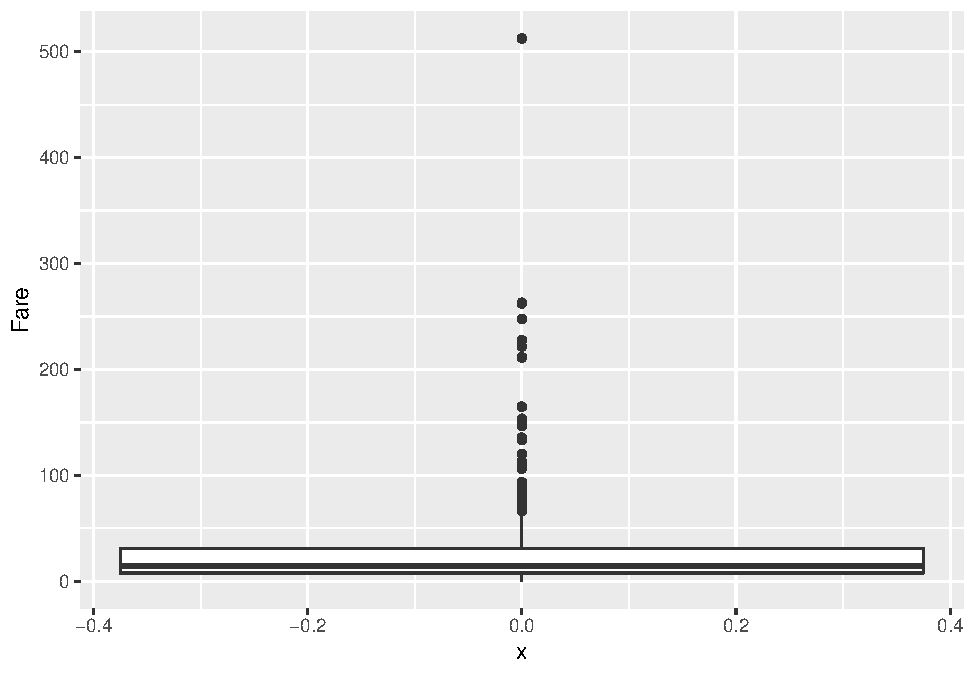
\includegraphics{m2851_PRA2_aruizplaza_rcotillas_files/figure-latex/unnamed-chunk-27-1.pdf}

Si observamos el boxplot realizado sobre la variable Fare, podríamos
observar que a partir de 60 Libras, se podrían considerar valores
extremos. Su tratamiento podría realizarse mediante la omisión de
aquellas observaciones asociadas a dichos valores extremos, la
asignación del valor máximo permitido sin ser outlier o incluso, o
categorizando la variable incluyendo todos los valores.

Finalmente, se opta por no considerar la existencia de valores extremos,
pues se tratan de valores que, aun siendo mayores que el resto de
observaciones, son posibles teniendo en cuenta que habían camarotes de
autentico lujo.Así pues, no se realiza tratamiento alguno sobre estos
casos. Además, usaremos un modelo robusto ante la existencia de valores
extremos.

\hypertarget{anuxe1lisis-de-los-datos.}{%
\section{.- Análisis de los datos.}\label{anuxe1lisis-de-los-datos.}}

\hypertarget{selecciuxf3n-de-los-grupos-de-datos-que-se-quieren-analizarcomparar-planificaciuxf3n-de-los-anuxe1lisis-a-aplicar.}{%
\subsection{.- Selección de los grupos de datos que se quieren
analizar/comparar (planificación de los análisis a
aplicar).}\label{selecciuxf3n-de-los-grupos-de-datos-que-se-quieren-analizarcomparar-planificaciuxf3n-de-los-anuxe1lisis-a-aplicar.}}

\textbf{Se preparan los datos para realizar los caontrastes de
hipostesis}

\begin{Shaded}
\begin{Highlighting}[]
\NormalTok{dfTrain.mujer <-}\StringTok{ }\NormalTok{dfTrain_fact[dfTrain_fact}\OperatorTok{$}\NormalTok{Sex }\OperatorTok{==}\StringTok{ "1"}\NormalTok{,]}\OperatorTok{$}\NormalTok{Survived}
\NormalTok{dfTrain.hombre <-}\StringTok{ }\NormalTok{dfTrain_fact[dfTrain_fact}\OperatorTok{$}\NormalTok{Sex }\OperatorTok{==}\StringTok{ "2"}\NormalTok{,]}\OperatorTok{$}\NormalTok{Survived}
\NormalTok{dfTrain.niños =}\StringTok{ }\NormalTok{dfTrain_fact[dfTrain_fact}\OperatorTok{$}\NormalTok{Age }\OperatorTok{==}\StringTok{ "1"} \OperatorTok{|}\StringTok{ }\NormalTok{dfTrain_fact}\OperatorTok{$}\NormalTok{Age }\OperatorTok{==}\StringTok{ "2"}\NormalTok{,]}\OperatorTok{$}\NormalTok{Survived}
\NormalTok{dfTrain.adultos =}\StringTok{ }\NormalTok{dfTrain_fact[dfTrain_fact}\OperatorTok{$}\NormalTok{Age }\OperatorTok{!=}\StringTok{ "1"} \OperatorTok{&}\StringTok{ }\NormalTok{dfTrain_fact}\OperatorTok{$}\NormalTok{Age }\OperatorTok{!=}\StringTok{ "2"}\NormalTok{,]}\OperatorTok{$}\NormalTok{Survived}
\end{Highlighting}
\end{Shaded}

\hypertarget{comprobaciuxf3n-de-la-normalidad-y-homogeneidad-de-la-varianza.}{%
\subsection{.- Comprobación de la normalidad y homogeneidad de la
varianza.}\label{comprobaciuxf3n-de-la-normalidad-y-homogeneidad-de-la-varianza.}}

\begin{Shaded}
\begin{Highlighting}[]
\NormalTok{alpha =}\StringTok{ }\FloatTok{0.05}
\NormalTok{col.names =}\StringTok{ }\KeywordTok{colnames}\NormalTok{(dfTrain_fact)}

\ControlFlowTok{for}\NormalTok{ (i }\ControlFlowTok{in} \DecValTok{1}\OperatorTok{:}\KeywordTok{ncol}\NormalTok{(dfTrain_fact)) \{}
  \ControlFlowTok{if}\NormalTok{ (i }\OperatorTok{==}\StringTok{ }\DecValTok{1}\NormalTok{) }
    \KeywordTok{cat}\NormalTok{(}\StringTok{"Variables que no siguen una distribución normal:}\CharTok{\textbackslash{}n}\StringTok{"}\NormalTok{)}
  \ControlFlowTok{if}\NormalTok{ (}\KeywordTok{is.integer}\NormalTok{(dfTrain_fact[,i]) }\OperatorTok{|}\StringTok{ }\KeywordTok{is.numeric}\NormalTok{(dfTrain_fact[,i])) \{}
\NormalTok{    p_val =}\StringTok{ }\KeywordTok{ad.test}\NormalTok{(dfTrain_fact[,i])}\OperatorTok{$}\NormalTok{p.value}
    \ControlFlowTok{if}\NormalTok{ (p_val }\OperatorTok{<}\StringTok{ }\NormalTok{alpha) \{}
      \KeywordTok{cat}\NormalTok{(col.names[i])}
      \CommentTok{# Format output}
      \ControlFlowTok{if}\NormalTok{ (i }\OperatorTok{<}\StringTok{ }\KeywordTok{ncol}\NormalTok{(dfTrain_fact) }\OperatorTok{-}\StringTok{ }\DecValTok{1}\NormalTok{) }
        \KeywordTok{cat}\NormalTok{(}\StringTok{", "}\NormalTok{)}
      \ControlFlowTok{if}\NormalTok{ (i }\OperatorTok\StringTok{ }\DecValTok{3} \OperatorTok{==}\StringTok{ }\DecValTok{0}\NormalTok{) }
        \KeywordTok{cat}\NormalTok{(}\StringTok{"}\CharTok{\textbackslash{}n}\StringTok{"}\NormalTok{)}
\NormalTok{    \}}
\NormalTok{  \}}
\NormalTok{\}}
\end{Highlighting}
\end{Shaded}

\begin{verbatim}
## Variables que no siguen una distribución normal:
## Survived, Pclass, Sex, 
## Age, SibSp, Parch, 
## Fare, EmbarkedSector
\end{verbatim}

Ahora Estudiamos la homogeneidad de varianzas mediante la aplicacion un
test de Fligner-Killeen, en este caso estudiamos la homogeneidad de los
grupos formados por los supervivientes y los no supervivientes con
respecto al precio del tiket.

\begin{Shaded}
\begin{Highlighting}[]
\KeywordTok{fligner.test}\NormalTok{(Fare }\OperatorTok{~}\StringTok{ }\NormalTok{Survived, }\DataTypeTok{data =}\NormalTok{ dfTrain_fact)}
\end{Highlighting}
\end{Shaded}

\begin{verbatim}
## 
##  Fligner-Killeen test of homogeneity of variances
## 
## data:  Fare by Survived
## Fligner-Killeen:med chi-squared = 96.253, df = 1, p-value < 2.2e-16
\end{verbatim}

como el p valor es \textless{} 0,05 rechazamos la hipotesis de que las
varianzas de ambas muestras sean homogéneas

\hypertarget{aplicaciuxf3n-de-pruebas-estaduxedsticas-para-comparar-los-grupos-de-datos.-en-funciuxf3n-de-los-datos-y-el-objetivo-del-estudio-aplicar-pruebas-de-contraste-de-hipuxf3tesis-correlaciones-regresiones-etc.-aplicar-al-menos-tres-muxe9todos-de-anuxe1lisis-diferentes.}{%
\subsection{.- Aplicación de pruebas estadísticas para comparar los
grupos de datos. En función de los datos y el objetivo del estudio,
aplicar pruebas de contraste de hipótesis, correlaciones, regresiones,
etc. Aplicar al menos tres métodos de análisis
diferentes.}\label{aplicaciuxf3n-de-pruebas-estaduxedsticas-para-comparar-los-grupos-de-datos.-en-funciuxf3n-de-los-datos-y-el-objetivo-del-estudio-aplicar-pruebas-de-contraste-de-hipuxf3tesis-correlaciones-regresiones-etc.-aplicar-al-menos-tres-muxe9todos-de-anuxe1lisis-diferentes.}}

\textbf{¿Que variables influyen mas en la supervivencia?}

\begin{Shaded}
\begin{Highlighting}[]
\NormalTok{correlation_mat }\OperatorTok{=}\NormalTok{ r.dfTrain_fact.corr()}
\NormalTok{sns.heatmap(correlation_mat, annot }\OperatorTok{=} \VariableTok{True}\NormalTok{)}
\NormalTok{plt.show()}
\end{Highlighting}
\end{Shaded}

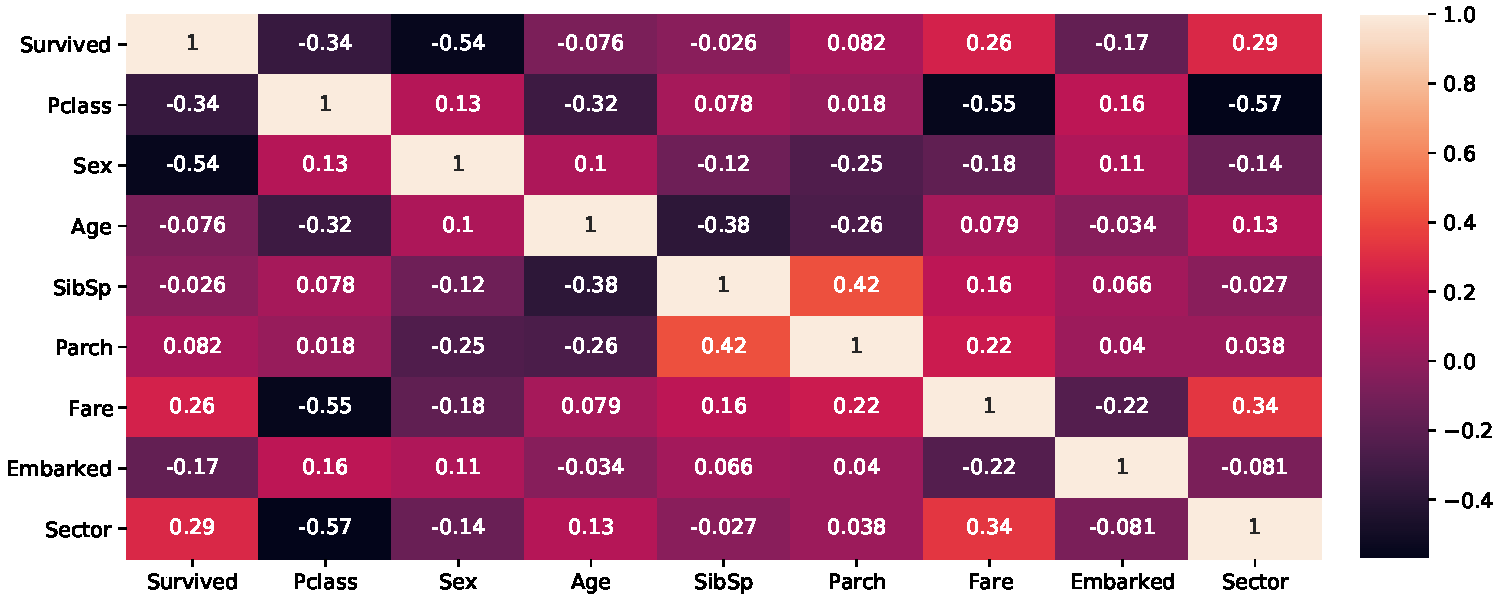
\includegraphics{m2851_PRA2_aruizplaza_rcotillas_files/figure-latex/unnamed-chunk-31-1.pdf}
Usando la matriz de correlacciones usada anteriormente, pero ya con el
dataset limpio, podemos concluir que las variables que más influyen en
la supervivencia son el sexo, la clase, y el Fare (en ese orden).

\textbf{¿la supervivencia es mayor en caso de ser niño o mujer (mujeres
y niños primero)?}

Se plantea el contraste de hipotesis de dos muestras sobre la diferencia
de medias, el cual es unilateral atendiendo a la formulación de la
hipótesis alternativa:

\(H_0: \mu_{h}-\mu_{m}=0\)

\(H_1: \mu_{h}-\mu_{m}<0\)

donde µh es la media de la población de la que se extrae la primera
muestra y µm es la media de la población de la que extrae la segunda.
Así, tomaremos α = 0, 05.

\begin{Shaded}
\begin{Highlighting}[]
\KeywordTok{t.test}\NormalTok{(dfTrain.hombre, dfTrain.mujer, }\DataTypeTok{alternative =} \StringTok{"less"}\NormalTok{)}
\end{Highlighting}
\end{Shaded}

\begin{verbatim}
## 
##  Welch Two Sample t-test
## 
## data:  dfTrain.hombre and dfTrain.mujer
## t = -18.672, df = 584.43, p-value < 2.2e-16
## alternative hypothesis: true difference in means is less than 0
## 95 percent confidence interval:
##        -Inf -0.5043259
## sample estimates:
## mean of x mean of y 
## 0.1889081 0.7420382
\end{verbatim}

Puesto que obtenemos un p-valor menor que el valor de significación
fijado, rechazamos la hipótesis nula. Por tanto, podemos concluir que
las mujeres tienen una supervivencia superior a la de los hombres.

Repetimos el procesos para los niños, en este caso consideramos niños a
los grupos de edad 1 y 2:

Formulamos el contraste de hipotesis:

\(H_0: \mu_{n}-\mu_{a}=0\)

\(H_1: \mu_{n}-\mu_{a}<0\)

Y lo realizamos de la misma manera que el anterior

\begin{Shaded}
\begin{Highlighting}[]
\KeywordTok{t.test}\NormalTok{(dfTrain.adultos, dfTrain.niños, }\DataTypeTok{alternative =} \StringTok{"less"}\NormalTok{)}
\end{Highlighting}
\end{Shaded}

\begin{verbatim}
## 
##  Welch Two Sample t-test
## 
## data:  dfTrain.adultos and dfTrain.niños
## t = -2.8207, df = 101.07, p-value = 0.002885
## alternative hypothesis: true difference in means is less than 0
## 95 percent confidence interval:
##         -Inf -0.06621461
## sample estimates:
## mean of x mean of y 
## 0.3684864 0.5294118
\end{verbatim}

Puesto que obtenemos un p-valor menor que el valor de significación
fijado, rechazamos la hipótesis nula. Por tanto, podemos concluir que
los niños tienen una supervivencia superior al resto, por lo tanto
podemos afirmar que se cumple el dicho ¡Mujeres y niños primero!

\hypertarget{modelo-predictivo}{%
\subsection{Modelo Predictivo}\label{modelo-predictivo}}

A continuación se plantea un modelo predictivo para intentar predecir la
supervivencia. En este caso se usará un random forest (anteriormente se
han probado otros modelos de clasificacion como la regresión logistica y
los arboles de decision pero con peores resultados) para evaluar el
modelo de una manera eficiente y evitar perder precisión con ello (ya
que no se cuenta con excesivos datos) se ha aplicado la técnica de
`cross-validation', dividiendo el dataset en 10 ``trozos''. No se ha
especificado el número de predictores para que sea el propio modelo el
que determine este dato.

\begin{Shaded}
\begin{Highlighting}[]
\KeywordTok{set.seed}\NormalTok{(}\DecValTok{14}\NormalTok{)}
\NormalTok{dfTrain_fact}\OperatorTok{$}\NormalTok{Survived =}\StringTok{ }\KeywordTok{as.factor}\NormalTok{(dfTrain_fact}\OperatorTok{$}\NormalTok{Survived)}

\CommentTok{# Definimos train control}
\NormalTok{train_control <-}\StringTok{ }\KeywordTok{trainControl}\NormalTok{(}\DataTypeTok{method=}\StringTok{'repeatedcv'}\NormalTok{, }
                              \DataTypeTok{number=}\DecValTok{10}\NormalTok{, }
                              \DataTypeTok{repeats=}\DecValTok{5}\NormalTok{)}

\CommentTok{# Entrenamos el modelo}
\NormalTok{(train.rpart <-}\StringTok{ }\KeywordTok{train}\NormalTok{(Survived }\OperatorTok{~}\StringTok{ }\NormalTok{Pclass }\OperatorTok{+}\StringTok{ }\NormalTok{Sex }\OperatorTok{+}\StringTok{ }\NormalTok{Age }\OperatorTok{+}\StringTok{ }\NormalTok{SibSp }\OperatorTok{+}\StringTok{ }\NormalTok{Parch }\OperatorTok{+}\StringTok{ }\NormalTok{Fare }\OperatorTok{+}\StringTok{ }\NormalTok{Embarked, }\CommentTok{#+ Sector, }
                    \DataTypeTok{data=}\NormalTok{dfTrain_fact, }
                    \DataTypeTok{method=}\StringTok{"rf"}\NormalTok{,}
                    \DataTypeTok{metric=}\StringTok{'Accuracy'}\NormalTok{, }
                    \DataTypeTok{trControl=}\NormalTok{train_control))}
\end{Highlighting}
\end{Shaded}

\begin{verbatim}
## Random Forest 
## 
## 891 samples
##   7 predictor
##   2 classes: '0', '1' 
## 
## No pre-processing
## Resampling: Cross-Validated (10 fold, repeated 5 times) 
## Summary of sample sizes: 802, 802, 802, 802, 802, 801, ... 
## Resampling results across tuning parameters:
## 
##   mtry  Accuracy   Kappa    
##   2     0.8284974  0.6231060
##   4     0.8309622  0.6341047
##   7     0.8235437  0.6191953
## 
## Accuracy was used to select the optimal model using the largest value.
## The final value used for the model was mtry = 4.
\end{verbatim}

\begin{Shaded}
\begin{Highlighting}[]
\CommentTok{# Imprimimos las puntuaciones de cross-validation}
\KeywordTok{summary}\NormalTok{(train.rpart)}
\end{Highlighting}
\end{Shaded}

\begin{verbatim}
##                 Length Class      Mode     
## call               4   -none-     call     
## type               1   -none-     character
## predicted        891   factor     numeric  
## err.rate        1500   -none-     numeric  
## confusion          6   -none-     numeric  
## votes           1782   matrix     numeric  
## oob.times        891   -none-     numeric  
## classes            2   -none-     character
## importance         7   -none-     numeric  
## importanceSD       0   -none-     NULL     
## localImportance    0   -none-     NULL     
## proximity          0   -none-     NULL     
## ntree              1   -none-     numeric  
## mtry               1   -none-     numeric  
## forest            14   -none-     list     
## y                891   factor     numeric  
## test               0   -none-     NULL     
## inbag              0   -none-     NULL     
## xNames             7   -none-     character
## problemType        1   -none-     character
## tuneValue          1   data.frame list     
## obsLevels          2   -none-     character
## param              0   -none-     list
\end{verbatim}

\begin{Shaded}
\begin{Highlighting}[]
\KeywordTok{summary}\NormalTok{(train.rpart}\OperatorTok{$}\NormalTok{finalModel)}
\end{Highlighting}
\end{Shaded}

\begin{verbatim}
##                 Length Class      Mode     
## call               4   -none-     call     
## type               1   -none-     character
## predicted        891   factor     numeric  
## err.rate        1500   -none-     numeric  
## confusion          6   -none-     numeric  
## votes           1782   matrix     numeric  
## oob.times        891   -none-     numeric  
## classes            2   -none-     character
## importance         7   -none-     numeric  
## importanceSD       0   -none-     NULL     
## localImportance    0   -none-     NULL     
## proximity          0   -none-     NULL     
## ntree              1   -none-     numeric  
## mtry               1   -none-     numeric  
## forest            14   -none-     list     
## y                891   factor     numeric  
## test               0   -none-     NULL     
## inbag              0   -none-     NULL     
## xNames             7   -none-     character
## problemType        1   -none-     character
## tuneValue          1   data.frame list     
## obsLevels          2   -none-     character
## param              0   -none-     list
\end{verbatim}

\begin{Shaded}
\begin{Highlighting}[]
\CommentTok{# Generamos la predicción}
\NormalTok{pred <-}\StringTok{ }\KeywordTok{predict}\NormalTok{(train.rpart, dfTrain_fact)}
\end{Highlighting}
\end{Shaded}

Podemos observar que el modelo arroja unos resultados decentes con
aproximadamente un 83\% de precisión (Finalmente se descarto el uso del
sector ya que este vajaba la precisión, esto es debido a gran numero de
nulos que tiene). El mejor resultado se ha obtenido usando 4
predictores.

\hypertarget{representaciuxf3n-de-los-resultados-a-partir-de-tablas-y-gruxe1ficas.}{%
\section{.- Representación de los resultados a partir de tablas y
gráficas.}\label{representaciuxf3n-de-los-resultados-a-partir-de-tablas-y-gruxe1ficas.}}

Visualizamos los datos que arroja el modelo:

\begin{Shaded}
\begin{Highlighting}[]
\KeywordTok{plot}\NormalTok{(train.rpart)}
\end{Highlighting}
\end{Shaded}

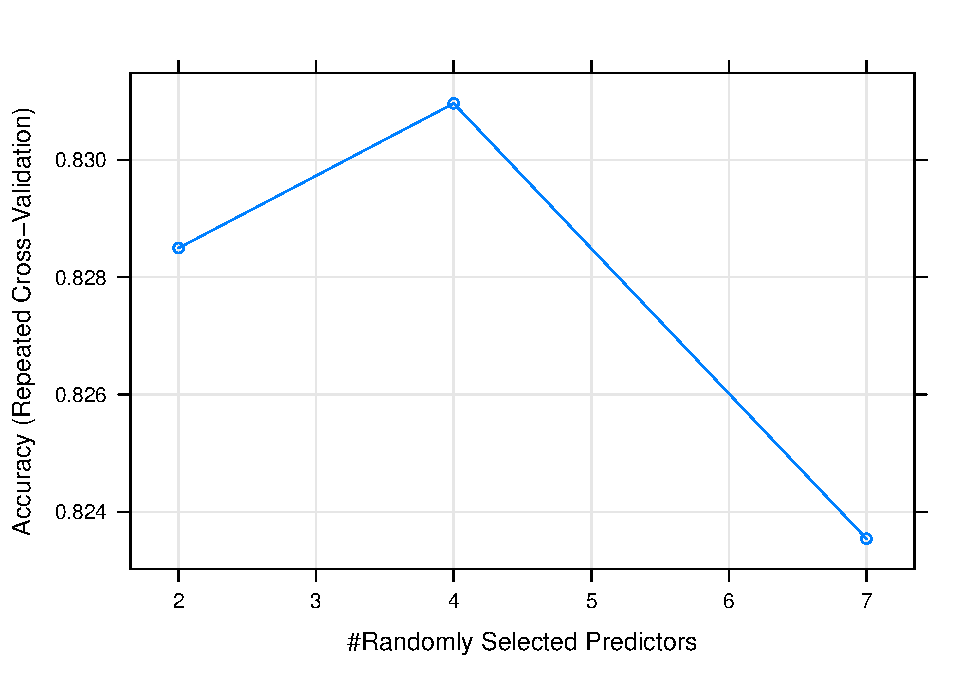
\includegraphics{m2851_PRA2_aruizplaza_rcotillas_files/figure-latex/unnamed-chunk-35-1.pdf}

\begin{Shaded}
\begin{Highlighting}[]
\KeywordTok{plot}\NormalTok{(train.rpart}\OperatorTok{$}\NormalTok{finalModel)}
\end{Highlighting}
\end{Shaded}

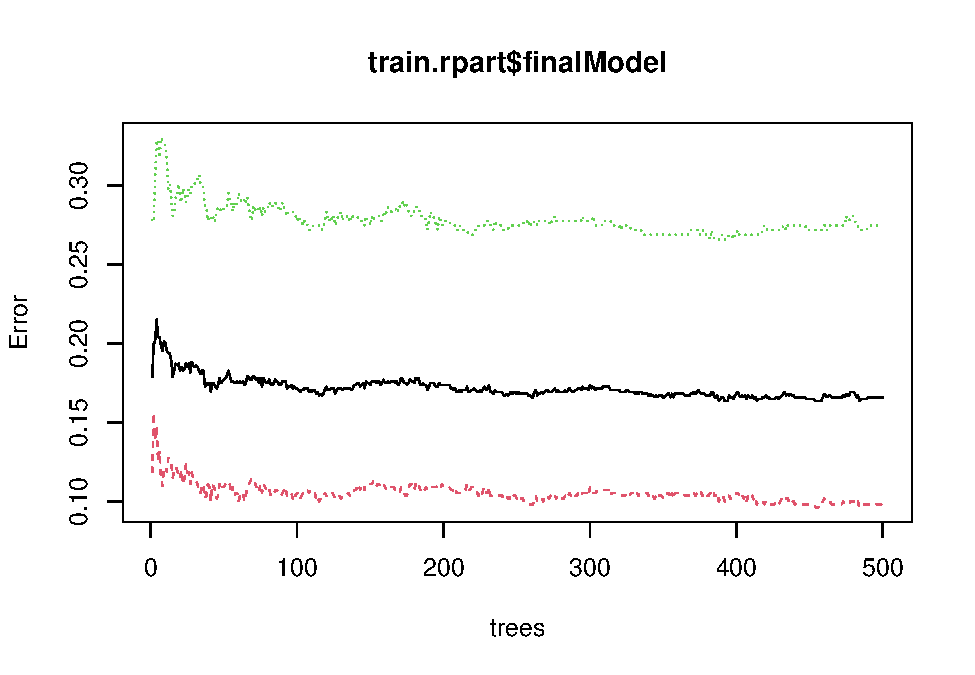
\includegraphics{m2851_PRA2_aruizplaza_rcotillas_files/figure-latex/unnamed-chunk-35-2.pdf}
\textbf{Se utiliza la siguiente función para generar el arbol de
decisión final.}

\begin{Shaded}
\begin{Highlighting}[]
\CommentTok{#Función optenida de https://shiring.github.io/machine_learning/2017/03/16/rf_plot_ggraph}
\NormalTok{tree_func <-}\StringTok{ }\ControlFlowTok{function}\NormalTok{(final_model, }
\NormalTok{                      tree_num) \{}
  
  \CommentTok{# get tree by index}
\NormalTok{  tree <-}\StringTok{ }\NormalTok{randomForest}\OperatorTok{::}\KeywordTok{getTree}\NormalTok{(final_model, }
                                \DataTypeTok{k =}\NormalTok{ tree_num, }
                                \DataTypeTok{labelVar =} \OtherTok{TRUE}\NormalTok{) }\OperatorTok
\StringTok{    }\NormalTok{tibble}\OperatorTok{::}\KeywordTok{rownames_to_column}\NormalTok{() }\OperatorTok
\StringTok{    }\CommentTok{# make leaf split points to NA, so the 0s won't get plotted}
\StringTok{    }\KeywordTok{mutate}\NormalTok{(}\StringTok{`}\DataTypeTok{split point}\StringTok{`}\NormalTok{ =}\StringTok{ }\KeywordTok{ifelse}\NormalTok{(}\KeywordTok{is.na}\NormalTok{(prediction), }\StringTok{`}\DataTypeTok{split point}\StringTok{`}\NormalTok{, }\OtherTok{NA}\NormalTok{))}
  
  \CommentTok{# prepare data frame for graph}
\NormalTok{  graph_frame <-}\StringTok{ }\KeywordTok{data.frame}\NormalTok{(}\DataTypeTok{from =} \KeywordTok{rep}\NormalTok{(tree}\OperatorTok{$}\NormalTok{rowname, }\DecValTok{2}\NormalTok{),}
                            \DataTypeTok{to =} \KeywordTok{c}\NormalTok{(tree}\OperatorTok{$}\StringTok{`}\DataTypeTok{left daughter}\StringTok{`}\NormalTok{, tree}\OperatorTok{$}\StringTok{`}\DataTypeTok{right daughter}\StringTok{`}\NormalTok{))}
  
  \CommentTok{# convert to graph and delete the last node that we don't want to plot}
\NormalTok{  graph <-}\StringTok{ }\KeywordTok{graph_from_data_frame}\NormalTok{(graph_frame) }\OperatorTok
\StringTok{    }\KeywordTok{delete_vertices}\NormalTok{(}\StringTok{"0"}\NormalTok{)}
  
  \CommentTok{# set node labels}
  \KeywordTok{V}\NormalTok{(graph)}\OperatorTok{$}\NormalTok{node_label <-}\StringTok{ }\KeywordTok{gsub}\NormalTok{(}\StringTok{"_"}\NormalTok{, }\StringTok{" "}\NormalTok{, }\KeywordTok{as.character}\NormalTok{(tree}\OperatorTok{$}\StringTok{`}\DataTypeTok{split var}\StringTok{`}\NormalTok{))}
  \KeywordTok{V}\NormalTok{(graph)}\OperatorTok{$}\NormalTok{leaf_label <-}\StringTok{ }\KeywordTok{as.character}\NormalTok{(tree}\OperatorTok{$}\NormalTok{prediction)}
  \KeywordTok{V}\NormalTok{(graph)}\OperatorTok{$}\NormalTok{split <-}\StringTok{ }\KeywordTok{as.character}\NormalTok{(}\KeywordTok{round}\NormalTok{(tree}\OperatorTok{$}\StringTok{`}\DataTypeTok{split point}\StringTok{`}\NormalTok{, }\DataTypeTok{digits =} \DecValTok{2}\NormalTok{))}
  
  \CommentTok{# plot}
\NormalTok{  plot <-}\StringTok{ }\KeywordTok{ggraph}\NormalTok{(graph, }\StringTok{'dendrogram'}\NormalTok{) }\OperatorTok{+}\StringTok{ }
\StringTok{    }\KeywordTok{theme_bw}\NormalTok{() }\OperatorTok{+}
\StringTok{    }\KeywordTok{geom_edge_link}\NormalTok{() }\OperatorTok{+}
\StringTok{    }\KeywordTok{geom_node_point}\NormalTok{() }\OperatorTok{+}
\StringTok{    }\KeywordTok{geom_node_text}\NormalTok{(}\KeywordTok{aes}\NormalTok{(}\DataTypeTok{label =}\NormalTok{ node_label), }\DataTypeTok{na.rm =} \OtherTok{TRUE}\NormalTok{, }\DataTypeTok{repel =} \OtherTok{TRUE}\NormalTok{) }\OperatorTok{+}
\StringTok{    }\KeywordTok{geom_node_label}\NormalTok{(}\KeywordTok{aes}\NormalTok{(}\DataTypeTok{label =}\NormalTok{ split), }\DataTypeTok{vjust =} \FloatTok{2.5}\NormalTok{, }\DataTypeTok{na.rm =} \OtherTok{TRUE}\NormalTok{, }\DataTypeTok{fill =} \StringTok{"white"}\NormalTok{) }\OperatorTok{+}
\StringTok{    }\KeywordTok{geom_node_label}\NormalTok{(}\KeywordTok{aes}\NormalTok{(}\DataTypeTok{label =}\NormalTok{ leaf_label, }\DataTypeTok{fill =}\NormalTok{ leaf_label), }\DataTypeTok{na.rm =} \OtherTok{TRUE}\NormalTok{, }
                    \DataTypeTok{repel =} \OtherTok{TRUE}\NormalTok{, }\DataTypeTok{colour =} \StringTok{"white"}\NormalTok{, }\DataTypeTok{fontface =} \StringTok{"bold"}\NormalTok{, }\DataTypeTok{show.legend =} \OtherTok{FALSE}\NormalTok{) }\OperatorTok{+}
\StringTok{    }\KeywordTok{theme}\NormalTok{(}\DataTypeTok{panel.grid.minor =} \KeywordTok{element_blank}\NormalTok{(),}
          \DataTypeTok{panel.grid.major =} \KeywordTok{element_blank}\NormalTok{(),}
          \DataTypeTok{panel.background =} \KeywordTok{element_blank}\NormalTok{(),}
          \DataTypeTok{plot.background =} \KeywordTok{element_rect}\NormalTok{(}\DataTypeTok{fill =} \StringTok{"white"}\NormalTok{),}
          \DataTypeTok{panel.border =} \KeywordTok{element_blank}\NormalTok{(),}
          \DataTypeTok{axis.line =} \KeywordTok{element_blank}\NormalTok{(),}
          \DataTypeTok{axis.text.x =} \KeywordTok{element_blank}\NormalTok{(),}
          \DataTypeTok{axis.text.y =} \KeywordTok{element_blank}\NormalTok{(),}
          \DataTypeTok{axis.ticks =} \KeywordTok{element_blank}\NormalTok{(),}
          \DataTypeTok{axis.title.x =} \KeywordTok{element_blank}\NormalTok{(),}
          \DataTypeTok{axis.title.y =} \KeywordTok{element_blank}\NormalTok{(),}
          \DataTypeTok{plot.title =} \KeywordTok{element_text}\NormalTok{(}\DataTypeTok{size =} \DecValTok{30}\NormalTok{))}
  
  \KeywordTok{print}\NormalTok{(plot)}
\NormalTok{\}}
\end{Highlighting}
\end{Shaded}

\textbf{Visualizamos el árbol de decisión resultante:}

\begin{Shaded}
\begin{Highlighting}[]
\NormalTok{tree_num <-}\StringTok{ }\KeywordTok{which}\NormalTok{(train.rpart}\OperatorTok{$}\NormalTok{finalModel}\OperatorTok{$}\NormalTok{forest}\OperatorTok{$}\NormalTok{ndbigtree }\OperatorTok{==}\StringTok{ }\KeywordTok{min}\NormalTok{(train.rpart}\OperatorTok{$}\NormalTok{finalModel}\OperatorTok{$}\NormalTok{forest}\OperatorTok{$}\NormalTok{ndbigtree))}
\KeywordTok{tree_func}\NormalTok{(}\DataTypeTok{final_model =}\NormalTok{ train.rpart}\OperatorTok{$}\NormalTok{finalModel, tree_num)}
\end{Highlighting}
\end{Shaded}

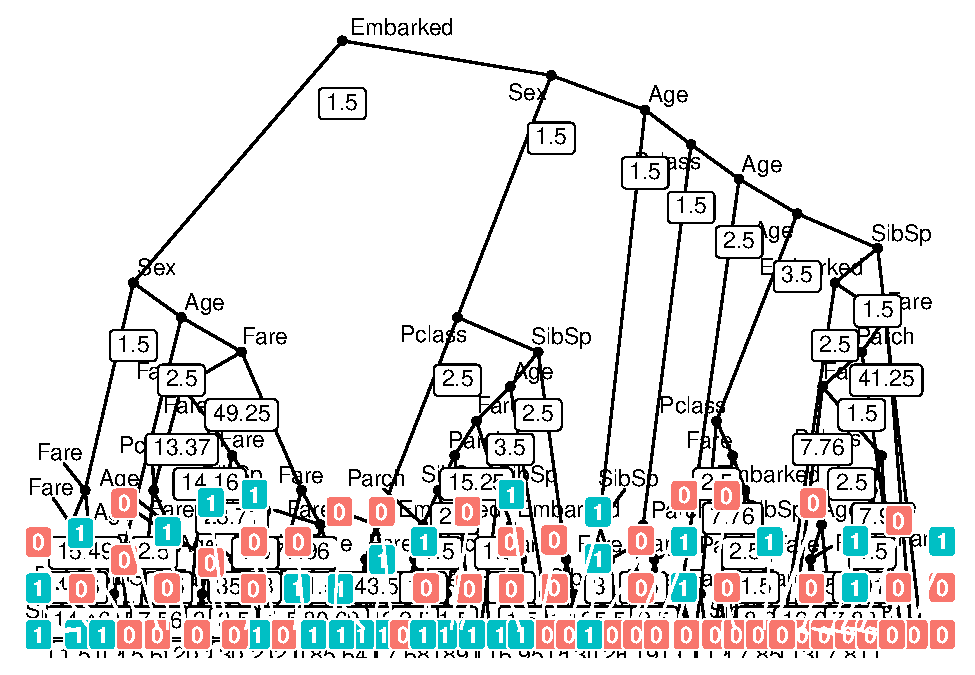
\includegraphics{m2851_PRA2_aruizplaza_rcotillas_files/figure-latex/unnamed-chunk-37-1.pdf}

\textbf{A continuación analizamos la matriz de confusión:}

\begin{Shaded}
\begin{Highlighting}[]
\CommentTok{#Función https://stackoverrun.com/es/q/6546365}
\NormalTok{draw_confusion_matrix <-}\StringTok{ }\ControlFlowTok{function}\NormalTok{(cm) \{}

     \KeywordTok{layout}\NormalTok{(}\KeywordTok{matrix}\NormalTok{(}\KeywordTok{c}\NormalTok{(}\DecValTok{1}\NormalTok{,}\DecValTok{1}\NormalTok{,}\DecValTok{2}\NormalTok{)))}
     \KeywordTok{par}\NormalTok{(}\DataTypeTok{mar=}\KeywordTok{c}\NormalTok{(}\DecValTok{2}\NormalTok{,}\DecValTok{2}\NormalTok{,}\DecValTok{2}\NormalTok{,}\DecValTok{2}\NormalTok{))}
     \KeywordTok{plot}\NormalTok{(}\KeywordTok{c}\NormalTok{(}\DecValTok{100}\NormalTok{, }\DecValTok{345}\NormalTok{), }\KeywordTok{c}\NormalTok{(}\DecValTok{300}\NormalTok{, }\DecValTok{450}\NormalTok{), }\DataTypeTok{type =} \StringTok{"n"}\NormalTok{, }\DataTypeTok{xlab=}\StringTok{""}\NormalTok{, }\DataTypeTok{ylab=}\StringTok{""}\NormalTok{, }\DataTypeTok{xaxt=}\StringTok{'n'}\NormalTok{, }\DataTypeTok{yaxt=}\StringTok{'n'}\NormalTok{)}
     \KeywordTok{title}\NormalTok{(}\StringTok{'CONFUSION MATRIX'}\NormalTok{, }\DataTypeTok{cex.main=}\DecValTok{2}\NormalTok{)}

     \CommentTok{# create the matrix }
     \KeywordTok{rect}\NormalTok{(}\DecValTok{150}\NormalTok{, }\DecValTok{430}\NormalTok{, }\DecValTok{240}\NormalTok{, }\DecValTok{370}\NormalTok{, }\DataTypeTok{col=}\StringTok{'#3F97D0'}\NormalTok{)}
     \KeywordTok{text}\NormalTok{(}\DecValTok{195}\NormalTok{, }\DecValTok{435}\NormalTok{, }\StringTok{'Class1'}\NormalTok{, }\DataTypeTok{cex=}\FloatTok{1.2}\NormalTok{)}
     \KeywordTok{rect}\NormalTok{(}\DecValTok{250}\NormalTok{, }\DecValTok{430}\NormalTok{, }\DecValTok{340}\NormalTok{, }\DecValTok{370}\NormalTok{, }\DataTypeTok{col=}\StringTok{'#F7AD50'}\NormalTok{)}
     \KeywordTok{text}\NormalTok{(}\DecValTok{295}\NormalTok{, }\DecValTok{435}\NormalTok{, }\StringTok{'Class2'}\NormalTok{, }\DataTypeTok{cex=}\FloatTok{1.2}\NormalTok{)}
     \KeywordTok{text}\NormalTok{(}\DecValTok{125}\NormalTok{, }\DecValTok{370}\NormalTok{, }\StringTok{'Predicted'}\NormalTok{, }\DataTypeTok{cex=}\FloatTok{1.3}\NormalTok{, }\DataTypeTok{srt=}\DecValTok{90}\NormalTok{, }\DataTypeTok{font=}\DecValTok{2}\NormalTok{)}
     \KeywordTok{text}\NormalTok{(}\DecValTok{245}\NormalTok{, }\DecValTok{450}\NormalTok{, }\StringTok{'Actual'}\NormalTok{, }\DataTypeTok{cex=}\FloatTok{1.3}\NormalTok{, }\DataTypeTok{font=}\DecValTok{2}\NormalTok{)}
     \KeywordTok{rect}\NormalTok{(}\DecValTok{150}\NormalTok{, }\DecValTok{305}\NormalTok{, }\DecValTok{240}\NormalTok{, }\DecValTok{365}\NormalTok{, }\DataTypeTok{col=}\StringTok{'#F7AD50'}\NormalTok{)}
     \KeywordTok{rect}\NormalTok{(}\DecValTok{250}\NormalTok{, }\DecValTok{305}\NormalTok{, }\DecValTok{340}\NormalTok{, }\DecValTok{365}\NormalTok{, }\DataTypeTok{col=}\StringTok{'#3F97D0'}\NormalTok{)}
     \KeywordTok{text}\NormalTok{(}\DecValTok{140}\NormalTok{, }\DecValTok{400}\NormalTok{, }\StringTok{'Class1'}\NormalTok{, }\DataTypeTok{cex=}\FloatTok{1.2}\NormalTok{, }\DataTypeTok{srt=}\DecValTok{90}\NormalTok{)}
     \KeywordTok{text}\NormalTok{(}\DecValTok{140}\NormalTok{, }\DecValTok{335}\NormalTok{, }\StringTok{'Class2'}\NormalTok{, }\DataTypeTok{cex=}\FloatTok{1.2}\NormalTok{, }\DataTypeTok{srt=}\DecValTok{90}\NormalTok{)}

     \CommentTok{# add in the cm results }
\NormalTok{     res <-}\StringTok{ }\KeywordTok{as.numeric}\NormalTok{(cm}\OperatorTok{$}\NormalTok{table)}
     \KeywordTok{text}\NormalTok{(}\DecValTok{195}\NormalTok{, }\DecValTok{400}\NormalTok{, res[}\DecValTok{1}\NormalTok{], }\DataTypeTok{cex=}\FloatTok{1.6}\NormalTok{, }\DataTypeTok{font=}\DecValTok{2}\NormalTok{, }\DataTypeTok{col=}\StringTok{'white'}\NormalTok{)}
     \KeywordTok{text}\NormalTok{(}\DecValTok{195}\NormalTok{, }\DecValTok{335}\NormalTok{, res[}\DecValTok{2}\NormalTok{], }\DataTypeTok{cex=}\FloatTok{1.6}\NormalTok{, }\DataTypeTok{font=}\DecValTok{2}\NormalTok{, }\DataTypeTok{col=}\StringTok{'white'}\NormalTok{)}
     \KeywordTok{text}\NormalTok{(}\DecValTok{295}\NormalTok{, }\DecValTok{400}\NormalTok{, res[}\DecValTok{3}\NormalTok{], }\DataTypeTok{cex=}\FloatTok{1.6}\NormalTok{, }\DataTypeTok{font=}\DecValTok{2}\NormalTok{, }\DataTypeTok{col=}\StringTok{'white'}\NormalTok{)}
     \KeywordTok{text}\NormalTok{(}\DecValTok{295}\NormalTok{, }\DecValTok{335}\NormalTok{, res[}\DecValTok{4}\NormalTok{], }\DataTypeTok{cex=}\FloatTok{1.6}\NormalTok{, }\DataTypeTok{font=}\DecValTok{2}\NormalTok{, }\DataTypeTok{col=}\StringTok{'white'}\NormalTok{)}

     \CommentTok{# add in the specifics }
     \KeywordTok{plot}\NormalTok{(}\KeywordTok{c}\NormalTok{(}\DecValTok{100}\NormalTok{, }\DecValTok{0}\NormalTok{), }\KeywordTok{c}\NormalTok{(}\DecValTok{100}\NormalTok{, }\DecValTok{0}\NormalTok{), }\DataTypeTok{type =} \StringTok{"n"}\NormalTok{, }\DataTypeTok{xlab=}\StringTok{""}\NormalTok{, }\DataTypeTok{ylab=}\StringTok{""}\NormalTok{, }\DataTypeTok{main =} \StringTok{"DETAILS"}\NormalTok{, }\DataTypeTok{xaxt=}\StringTok{'n'}\NormalTok{, }\DataTypeTok{yaxt=}\StringTok{'n'}\NormalTok{)}
     \KeywordTok{text}\NormalTok{(}\DecValTok{10}\NormalTok{, }\DecValTok{85}\NormalTok{, }\KeywordTok{names}\NormalTok{(cm}\OperatorTok{$}\NormalTok{byClass[}\DecValTok{1}\NormalTok{]), }\DataTypeTok{cex=}\FloatTok{1.2}\NormalTok{, }\DataTypeTok{font=}\DecValTok{2}\NormalTok{)}
     \KeywordTok{text}\NormalTok{(}\DecValTok{10}\NormalTok{, }\DecValTok{70}\NormalTok{, }\KeywordTok{round}\NormalTok{(}\KeywordTok{as.numeric}\NormalTok{(cm}\OperatorTok{$}\NormalTok{byClass[}\DecValTok{1}\NormalTok{]), }\DecValTok{3}\NormalTok{), }\DataTypeTok{cex=}\FloatTok{1.2}\NormalTok{)}
     \KeywordTok{text}\NormalTok{(}\DecValTok{30}\NormalTok{, }\DecValTok{85}\NormalTok{, }\KeywordTok{names}\NormalTok{(cm}\OperatorTok{$}\NormalTok{byClass[}\DecValTok{2}\NormalTok{]), }\DataTypeTok{cex=}\FloatTok{1.2}\NormalTok{, }\DataTypeTok{font=}\DecValTok{2}\NormalTok{)}
     \KeywordTok{text}\NormalTok{(}\DecValTok{30}\NormalTok{, }\DecValTok{70}\NormalTok{, }\KeywordTok{round}\NormalTok{(}\KeywordTok{as.numeric}\NormalTok{(cm}\OperatorTok{$}\NormalTok{byClass[}\DecValTok{2}\NormalTok{]), }\DecValTok{3}\NormalTok{), }\DataTypeTok{cex=}\FloatTok{1.2}\NormalTok{)}
     \KeywordTok{text}\NormalTok{(}\DecValTok{50}\NormalTok{, }\DecValTok{85}\NormalTok{, }\KeywordTok{names}\NormalTok{(cm}\OperatorTok{$}\NormalTok{byClass[}\DecValTok{5}\NormalTok{]), }\DataTypeTok{cex=}\FloatTok{1.2}\NormalTok{, }\DataTypeTok{font=}\DecValTok{2}\NormalTok{)}
     \KeywordTok{text}\NormalTok{(}\DecValTok{50}\NormalTok{, }\DecValTok{70}\NormalTok{, }\KeywordTok{round}\NormalTok{(}\KeywordTok{as.numeric}\NormalTok{(cm}\OperatorTok{$}\NormalTok{byClass[}\DecValTok{5}\NormalTok{]), }\DecValTok{3}\NormalTok{), }\DataTypeTok{cex=}\FloatTok{1.2}\NormalTok{)}
     \KeywordTok{text}\NormalTok{(}\DecValTok{70}\NormalTok{, }\DecValTok{85}\NormalTok{, }\KeywordTok{names}\NormalTok{(cm}\OperatorTok{$}\NormalTok{byClass[}\DecValTok{6}\NormalTok{]), }\DataTypeTok{cex=}\FloatTok{1.2}\NormalTok{, }\DataTypeTok{font=}\DecValTok{2}\NormalTok{)}
     \KeywordTok{text}\NormalTok{(}\DecValTok{70}\NormalTok{, }\DecValTok{70}\NormalTok{, }\KeywordTok{round}\NormalTok{(}\KeywordTok{as.numeric}\NormalTok{(cm}\OperatorTok{$}\NormalTok{byClass[}\DecValTok{6}\NormalTok{]), }\DecValTok{3}\NormalTok{), }\DataTypeTok{cex=}\FloatTok{1.2}\NormalTok{)}
     \KeywordTok{text}\NormalTok{(}\DecValTok{90}\NormalTok{, }\DecValTok{85}\NormalTok{, }\KeywordTok{names}\NormalTok{(cm}\OperatorTok{$}\NormalTok{byClass[}\DecValTok{7}\NormalTok{]), }\DataTypeTok{cex=}\FloatTok{1.2}\NormalTok{, }\DataTypeTok{font=}\DecValTok{2}\NormalTok{)}
     \KeywordTok{text}\NormalTok{(}\DecValTok{90}\NormalTok{, }\DecValTok{70}\NormalTok{, }\KeywordTok{round}\NormalTok{(}\KeywordTok{as.numeric}\NormalTok{(cm}\OperatorTok{$}\NormalTok{byClass[}\DecValTok{7}\NormalTok{]), }\DecValTok{3}\NormalTok{), }\DataTypeTok{cex=}\FloatTok{1.2}\NormalTok{)}

     \CommentTok{# add in the accuracy information }
     \KeywordTok{text}\NormalTok{(}\DecValTok{30}\NormalTok{, }\DecValTok{35}\NormalTok{, }\KeywordTok{names}\NormalTok{(cm}\OperatorTok{$}\NormalTok{overall[}\DecValTok{1}\NormalTok{]), }\DataTypeTok{cex=}\FloatTok{1.5}\NormalTok{, }\DataTypeTok{font=}\DecValTok{2}\NormalTok{)}
     \KeywordTok{text}\NormalTok{(}\DecValTok{30}\NormalTok{, }\DecValTok{20}\NormalTok{, }\KeywordTok{round}\NormalTok{(}\KeywordTok{as.numeric}\NormalTok{(cm}\OperatorTok{$}\NormalTok{overall[}\DecValTok{1}\NormalTok{]), }\DecValTok{3}\NormalTok{), }\DataTypeTok{cex=}\FloatTok{1.4}\NormalTok{)}
     \KeywordTok{text}\NormalTok{(}\DecValTok{70}\NormalTok{, }\DecValTok{35}\NormalTok{, }\KeywordTok{names}\NormalTok{(cm}\OperatorTok{$}\NormalTok{overall[}\DecValTok{2}\NormalTok{]), }\DataTypeTok{cex=}\FloatTok{1.5}\NormalTok{, }\DataTypeTok{font=}\DecValTok{2}\NormalTok{)}
     \KeywordTok{text}\NormalTok{(}\DecValTok{70}\NormalTok{, }\DecValTok{20}\NormalTok{, }\KeywordTok{round}\NormalTok{(}\KeywordTok{as.numeric}\NormalTok{(cm}\OperatorTok{$}\NormalTok{overall[}\DecValTok{2}\NormalTok{]), }\DecValTok{3}\NormalTok{), }\DataTypeTok{cex=}\FloatTok{1.4}\NormalTok{)}
\NormalTok{\}  }

\NormalTok{cm <-}\StringTok{ }\KeywordTok{confusionMatrix}\NormalTok{(pred, train.rpart}\OperatorTok{$}\NormalTok{trainingData}\OperatorTok{$}\NormalTok{.outcome, }\DataTypeTok{mode =} \StringTok{"everything"}\NormalTok{)}
\KeywordTok{draw_confusion_matrix}\NormalTok{(cm)}
\end{Highlighting}
\end{Shaded}

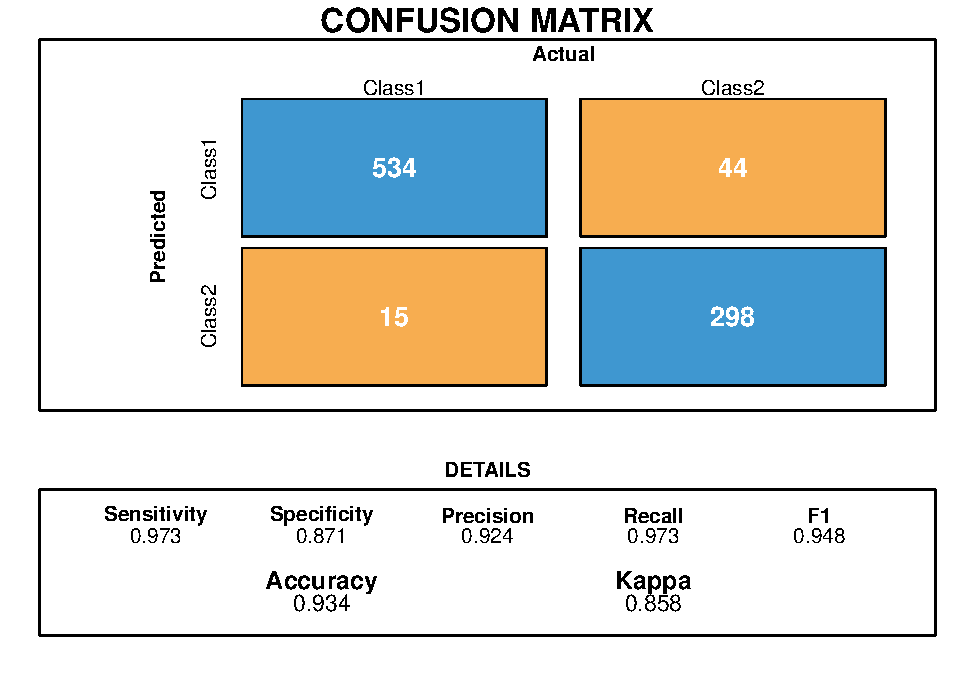
\includegraphics{m2851_PRA2_aruizplaza_rcotillas_files/figure-latex/unnamed-chunk-38-1.pdf}

Esta matriz de confusión arroja mejores resultados a los obtenidos
mediante el proceso de `Cross-Validation'(CV). Esto es debido a que se
estan usando todos los datos para confeccionarla (ya que no hemos
dividido el dataset en train y test). Por lo tanto es mucho más
confiable la accuracy optenida en el proceso de CV, sin embargo si que
vale para darnos una idea de las otras métricas.

Por otro lado vamos a ver las siguientes gráficas referentes a los
contrastes de hipótesis realizados con anterioridad donde se puede
observar gráficamente cómo la supervivecia es mucho mayor en el caso de
las mujeres y los niños.

\begin{Shaded}
\begin{Highlighting}[]
\NormalTok{dfTrain_cat}\OperatorTok{$}\NormalTok{child <-}\StringTok{ }\KeywordTok{cut}\NormalTok{(dfTrain}\OperatorTok{$}\NormalTok{Age, }\KeywordTok{c}\NormalTok{(}\DecValTok{0}\NormalTok{,}\DecValTok{13}\NormalTok{,}\DecValTok{100}\NormalTok{), }\DataTypeTok{labels=}\KeywordTok{c}\NormalTok{(}\StringTok{"Child"}\NormalTok{, }\StringTok{"Adult"}\NormalTok{))}
\NormalTok{dfTrain_cat}\OperatorTok{$}\NormalTok{child[dfTrain_cat}\OperatorTok{$}\NormalTok{child }\OperatorTok{==}\StringTok{ "1"}\NormalTok{] <-}\StringTok{ "Child"}
\end{Highlighting}
\end{Shaded}

\begin{Shaded}
\begin{Highlighting}[]
\NormalTok{fig, axs }\OperatorTok{=}\NormalTok{ plt.subplots(ncols}\OperatorTok{=}\DecValTok{1}\NormalTok{, constrained_layout}\OperatorTok{=}\VariableTok{True}\NormalTok{, figsize}\OperatorTok{=}\NormalTok{(}\DecValTok{5}\NormalTok{,}\DecValTok{4}\NormalTok{))}
\NormalTok{sns.countplot(x}\OperatorTok{=}\StringTok{"child"}\NormalTok{, hue}\OperatorTok{=}\StringTok{'Survived'}\NormalTok{, data}\OperatorTok{=}\NormalTok{r.dfTrain_cat, ax}\OperatorTok{=}\NormalTok{axs).}\BuiltInTok{set}\NormalTok{(title}\OperatorTok{=}\StringTok{'Child with Survived'}\NormalTok{)}
\NormalTok{plt.show()}
\end{Highlighting}
\end{Shaded}

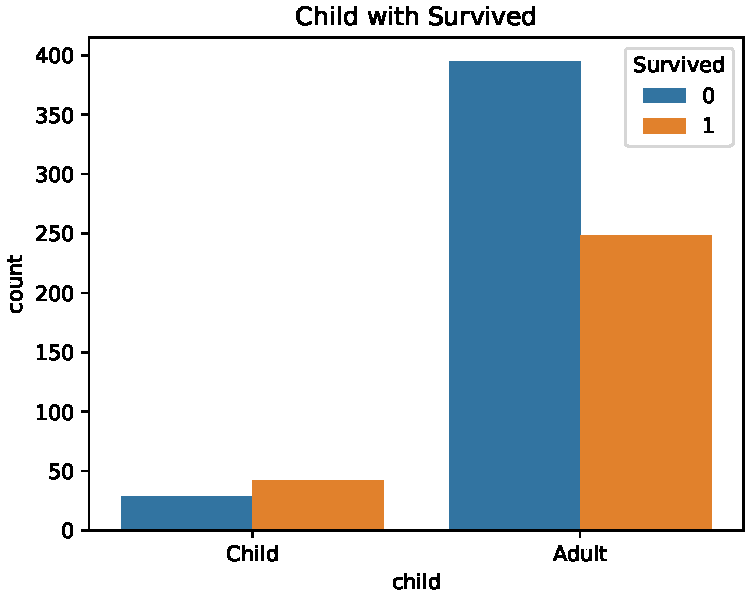
\includegraphics{m2851_PRA2_aruizplaza_rcotillas_files/figure-latex/unnamed-chunk-40-1.pdf}

\begin{Shaded}
\begin{Highlighting}[]
\NormalTok{fig, axs }\OperatorTok{=}\NormalTok{ plt.subplots(ncols}\OperatorTok{=}\DecValTok{1}\NormalTok{, constrained_layout}\OperatorTok{=}\VariableTok{True}\NormalTok{, figsize}\OperatorTok{=}\NormalTok{(}\DecValTok{5}\NormalTok{,}\DecValTok{4}\NormalTok{))}
\NormalTok{sns.countplot(x}\OperatorTok{=}\StringTok{"Sex"}\NormalTok{, hue}\OperatorTok{=}\StringTok{'Survived'}\NormalTok{, data}\OperatorTok{=}\NormalTok{r.dfTrain_cat, ax}\OperatorTok{=}\NormalTok{axs).}\BuiltInTok{set}\NormalTok{(title}\OperatorTok{=}\StringTok{'Sex with Survived'}\NormalTok{)}
\NormalTok{plt.show()}
\end{Highlighting}
\end{Shaded}

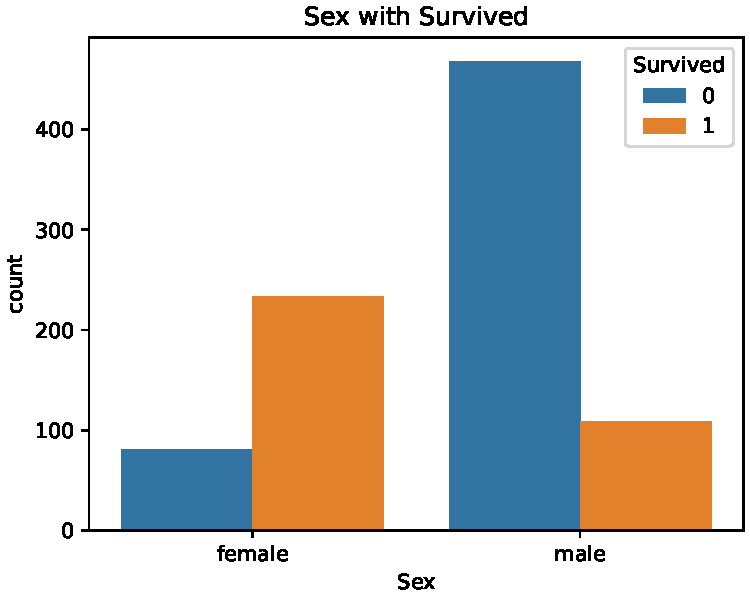
\includegraphics{m2851_PRA2_aruizplaza_rcotillas_files/figure-latex/unnamed-chunk-41-1.pdf}

\hypertarget{conclusiones}{%
\section{.- Conclusiones}\label{conclusiones}}

Al principio de la práctica se planteaban una serie de preguntas que se
han ido respondiendo en el transcurso de la misma.

A la pregunta de cuales son las variables más influyentes a la hora de
predecir la supervivencia, se respondió con un una tabla de correlación,
a la de si las mujeres y los niños tenían una supervivencia mayor, se
respondió con contrastes de hipótesis y a la pregunta de si se podía
predecir la supervivencia se aporto un modelo (random forest) para el
cual se usaron técnicas de validación cruzada para aprovechar mejor el
escaso dataset con el que nos encontramos.

Previo a estas pruebas estadísticas, se sometieron los datos a un
preprocesamiento para manejar los casos de elementos vacíos y outliers.
Para el caso de los elementos vacíos se opto por el uso de modelos de
predicción sencillos para evitar tener que eliminar las filas, excepto
en el caso de la columna Cabin, que si bien se optó por rellenar los
valores desconocidos con un valor por defecto, en la aplicación del
modelo se observo que no aportaba nada y finalmente se elimino de esté.
El caso de la variable Age es un caso especial ya que intentamos
predecirla usando un modelo complejo, pero nos encontramos un problema
de datos desbalanceados que finalmente se decidió no abordar y usar el
mismo modelo de vecinos más cercanos usado en las otras variables. Para
el caso de los outliers, se estudió categorizar la variable, pero
finalmente se optó por incluir los valores extremos en los análisis dado
que son valores totalmente posibles en un crucero y eliminarlos seria
eliminar del estudio los valores de lujo, además el modelo elegido es un
modelo muy robusto ante los outliers.

Por otro lado, hemos incluido constantes visualizaciones y comentarios
en cada proceso para que sea más fácil entender el dataset en un
principio y los resultados obtenidos de las pruebas.

Finalmente, creemos que se ha conseguido un modelo decente para predecir
la supervivencia, aunque se podría mejorar si se encontrara una manera
de usar mejor la variable cabin y hubieramos podido predecir con más
efectividad la edad.

\hypertarget{recursos}{%
\section{.- Recursos}\label{recursos}}

\begin{itemize}
\tightlist
\item
  Calvo M., Subirats L., Pérez D. (2019). Introducción a la limpieza y
  análisis de los datos. Editorial UOC.
\item
  Megan Squire (2015). Clean Data. Packt Publishing Ltd.
\item
  Jiawei Han, Micheine Kamber, Jian Pei (2012). Data mining: concepts
  and techniques.Morgan Kaufmann.
\item
  Jason W. Osborne (2010). Data Cleaning Basics: Best Practices in
  Dealing with Extreme Scores. Newborn and Infant Nursing Reviews; 10
  (1): pp.~1527-3369.
\item
  Peter Dalgaard (2008). Introductory statistics with R. Springer
  Science \& Business Media.
\item
  Wes McKinney (2012). Python for Data Analysis. O'Reilley Media, Inc.
\end{itemize}

\hypertarget{tabla-de-contribuciones}{%
\section{.- Tabla de contribuciones}\label{tabla-de-contribuciones}}

\begin{longtable}[]{@{}ll@{}}
\toprule
Contribuciones & Firma\tabularnewline
\midrule
\endhead
Investigación previa & aruizplaza, rcotillas\tabularnewline
Redacción de las respuestas & aruizplaza, rcotillas\tabularnewline
Desarrollo código & aruizplaza, rcotillas\tabularnewline
\bottomrule
\end{longtable}

\end{document}
